\documentclass[a4paper,12pt]{report}
\renewcommand\thechapter{\Roman{chapter}}
\usepackage[utf8]{inputenc}
\usepackage{kantlipsum}
\usepackage[calcwidth]{titlesec}
\usepackage{fix-cm} 
\usepackage[Sonny]{fncychap}
\usepackage{setspace}
\usepackage{natbib}
\usepackage{pdflscape}
\usepackage{float}
\usepackage{siunitx,booktabs}
\usepackage{pgfplotstable}
\usepackage{pgfplots}
\usepackage{subcaption}
\usepackage{lscape}
\usepackage{afterpage}
\usepackage{graphicx}
\usepackage[raggedrightboxes]{ragged2e}
\usepackage[bottom=3cm, right=2.5cm, left=2.5cm, top=3cm]{geometry}
\usepackage{changepage}
\usepackage{makecell}
\usepackage{colortbl}
%\usepackage{biblatex}
%\addbibresource{references.bib}
%\bibliographystyle{apacite}
\usepackage{pgf-pie}
\usepackage{lipsum}% For 'Lorem Ipsum' dummy text
\usepackage[pscoord]{eso-pic}% The zero point of the coordinate systemis the lower left corner of the page (the default).
\usepackage{xcolor}
\definecolor{findOptimalPartition}{HTML}{D7191C}
\definecolor{storeClusterComponent}{HTML}{FDAE61}
\definecolor{dbscan}{HTML}{ABDDA4}
\definecolor{constructCluster}{HTML}{2B83BA}
\usepackage{listings, caption, graphicx, array, url}
\lstset{frame=lines}
\lstset{escapeinside={<@}{@>}}
\lstset{showstringspaces=false}
\usepackage{tikz,forest}
\usetikzlibrary{arrows.meta}
\usetikzlibrary{shapes}
\usepackage{amsmath}
\usepackage{xspace}
\newcommand{\A}{\ensuremath{\mathcal{A}}\xspace}
\newcommand{\B}{\ensuremath{\mathcal{B}}\xspace}
\newcommand\pa[1]{\ensuremath{\left(#1\right)}}

\usepackage[toc,page]{appendix}

\newcommand{\placetextbox}[3]{% \placetextbox{<horizontal pos>}{<vertical pos>}{<stuff>}
  \setbox0=\hbox{#3}% Put <stuff> in a box
  \AddToShipoutPictureFG*{% Add <stuff> to current page foreground
    \put(\LenToUnit{#1\paperwidth},\LenToUnit{#2\paperheight}){\vtop{{\null}\makebox[0pt][c]{#3}}}%
  }%
}%

\pgfplotsset{
        compat=1.3,
    }
\pgfplotsset{compat=newest}
\usetikzlibrary{patterns}
\usepgfplotslibrary{fillbetween}
\sisetup{group-digits=false}

\doublespacing
\setlength{\parindent}{0pt}
\renewcommand{\baselinestretch}{1.3} 

\titleformat{\chapter}[display]{\Large}{\centering
  \MakeUppercase{\chaptername}\quad{\Huge\thechapter}}{10pt}{\titlerule[.5pt]\vspace{10pt}\centering
  \MakeUppercase}[\vspace{10pt}{\titlerule[.5pt]}]% <-- spacing of title bar
\titlespacing{\chapter}{0pt}{-50pt}{1cm}% <-- spacing of title bar


\usepackage{amsthm, amsmath, amssymb, mathtools, mathbbol}
\numberwithin{equation}{section}
\theoremstyle{definition}
\newtheorem{thm}{Theorem}[section]
\newtheorem{Def}[thm]{Definition}
\newtheorem{prob}[thm]{Problem}
\newtheorem{rem}[thm]{Remark}

%\usepackage{natbib}
\usepackage{graphicx}

\graphicspath{{graphics/}}

\begin{document}
\pagenumbering{gobble}

\begin{center}
\Large NATIONAL UNIVERSITY OF SINGAPORE\\ 
\Large Master's of Computing (General-Track) \\ [0.2in]

\includegraphics[width=10cm]{1.nus_logo_full-horizontal} \\
\Large {\bf Alpha Tree Search and Machine Learning Approaches to Optimising Real Estate Portfolios}\\ [0.5in]
Leong Wei Ming \\
Supervisor: Professor Liu Li Li \\
Examiner: Professor Chin Wei Ngan \\ [0.3in]
Department of Computer Science \\
Internal Capstone Project for AY2023/2024
\end{center}

\chapter*{Abstract}
An internal project about applying genetic algorithm to search for optimal alphas.    
State the major contribution:

\chapter*{Declaration}
\begin{center}{\large
I hereby declare that this project report is my original work and it has been written by me in its entirety. I have duly acknowledged all the sources of information which have been used in this report. \\[0.5in]
This report has also not been submitted for any degree in any university previously.
}

\chapter*{Acknowledgement}
{\large
I would like to thank Professor Liu Lili for her guidance, support and encouragement throughout the course of this project. Working with Professor Lili has been a great learning experience, getting to learn much more about machine learning and its applications to finance in solving some challenges faced by industry practitioners. \\[0.5in]
Also many thanks to Professor Chin Wei Ngan for taking the time out to assess this project.

}
\end{center}
\setcounter{secnumdepth}{3}
\setcounter{tocdepth}{3}


\tableofcontents


\setcounter{chapter}{1}
\renewcommand{\thechapter}{\arabic{chapter}}
\pagenumbering{arabic}
\setcounter{chapter}{0}
\setcounter{page}{0}
\chapter{Introduction}
The saying goes that once a profitable trading formula has been discovered and traded on by enough people, its profits will be eroded away and it will cease to be profitable. Traders and investors appear to be playing a never-ending game of "Hide-and-Seek" in search of profitable trading strategies. Due to the evolving nature of the financial markets, traditional financial time-series forecasting models which are static in nature are becoming less effective than Machine Learning models and dynamic algorithms in identifying the best investments (Sheth \& Manan, 2023). The success of Machine Learning has led to numerous research papers applying a myriad of Machine Learning techniques to predict stock prices (Obthong et.al., 2020). However, fewer papers apply these approaches in the Real Estate sector and these papers largely focus on future stock price prediction rather than portfolio allocation as a whole (Habab \& Kampouridis, 2024). Many of these papers also use price-volume data without fundamental financial data as inputs. In 2022, the global real estate sector was worth more than \$380 trillion and worth more than the global equity and bond markets combined (Tostevin \& Rushton, 2023), with approximately 893 listed Real Estate Investment Trusts (REITs) (Nareit, 2024). Hence, addressing the research gaps in this sector is particularly valuable.


\section{Problem Definition}
The aim of this report is to develop an effective real estate portfolio optimisation model that maximises profits, minimises risks and outperforms the market indexes with a sharpe ratio of more than 2. A novel approach of applying Genetic Algorithms to search for outperforming Alpha formulas, as well as, three Machine Learning models, namely, Multiple Linear Regression (MLR), Neural Networks (NN) and Long-Short Term Memory (LSTM) are used to construct models. A trading agent is also constructed to allocate funds to the portfolio based on the results from the models. The input data to the Machine Learning models will be extended beyond price-volume data to include fundamental stock data. The models will be trained on 10 years worth of real market data. Then, the performances of these approaches will be compared with traditional financial models and the market indexes.

\section{Motivations}
Interviews of traders and financial journalists have revealed that both technical and fundamental analysis are used for forecasting investments, for shorter and medium to long term investment horizons respectively (Oberlechner, 2001). Given that most investments in real estate are meant for the medium to long term, the lack of fundamental data inputs for REITs stock price predictions reveals a pressing need for fundamental data to be incorporated. \\ 

In the field of quantitative trading, quant firms seek to develop predictive algorithms for quantitative trading called "Alphas" that determine how capital is allocated to portfolios profitably (Tulchinsky, 2019). What began with investment experts manually constructing Alpha formulas has gradually been replaced with automated alpha mining techniques that employ Machine Learning algorithms (Wang et. al., 2023). There appears to be an opportunity to apply the concept of quantitative finance Alphas for Real Estate portfolio allocation. In addition, researchers have been inspired by Charles Darwin's theory of evolution (Ruse, 1975) to develop a Genetic Algorithm and have applied it in finance (Aguilar-Rivera et. al., 2015). Synthesising these two ideas, presents a new and innovative approach to use Genetic Algorithms to search for Alphas in the Real Estate sector. \\

Lastly, as most of past research is centered on price prediction, there is a need to develop trade execution logic to allocate portfolios based on these predictions.



\section{Major Contributions and Creativity}
The first major contribution of this project is the analysis on REITs stock datasets with more than 150 features of technical and fundamental indicators. This expands the dimensionality of the input training data significantly beyond price-volume features to incorporate REIT company data from financial statements. The comprehensive dataset covers 150 out of the total worldwide population of 893 REITs and includes up to 20 years of historical data.\\

Creativity is demonstrated in the writing of a Genetic Search Algorithm that searches for outperforming REIT Alphas. It resulted in the second major contribution of a trading model with superior returns that significantly outperforms the market indexes.\\ 

The third contribution is the implementation of a trading agent or trade execution logic that acts on individual REIT price predictions to allocate funds to selected REITS in a portfolio.\\

Overall, this research paper has expanded the body of knowledge on the application of Alphas and Machine Learning models in Optimising Real Estate Portfolios.

\titleformat{\chapter}[block]
  {\normalfont\huge\bfseries}{\thechapter.}{1em}{\Huge\centering}
\titlespacing*{\chapter}{0pt}{230pt}{0pt}
\setcounter{chapter}{0}
\renewcommand{\thechapter}{\Roman{chapter}}

\chapter{Background}


\titleformat{\chapter}[display]{\Large}{\centering
  \MakeUppercase{\chaptername}\quad{\Huge\thechapter}}{10pt}{\titlerule[.5pt]\vspace{10pt}\centering
  \MakeUppercase}[\vspace{10pt}{\titlerule[.5pt]}]% <-- spacing of title bar
\titlespacing{\chapter}{0pt}{-80pt}{1cm}% <-- spacing of title bar
\renewcommand{\thechapter}{\arabic{chapter}}

\pagenumbering{arabic}
\setcounter{page}{3}
\chapter{Financial Terminology and Concepts}
In order to better communicate ideas, the key financial terminologies and formulas are synthesised from Stephen Ross' Corporate Finance textbook (2021) and applied to the context of this paper. Particularly the difference between a stock, REIT and a portfolio, the difference between technical and fundamental analysis and the concept of Alphas. This builds the foundation for further discussions on the measures of portfolio performance, namely, profits/losses and the sharpe ratio. Other methods of analysis such as sentiment and macro-economic analysis is also briefly discussed. 
\section{Key Terms}
The relationship between stocks, REITs and Portfolios can be illustrated in the figure below.
\begin{figure}[H]
  \centerline{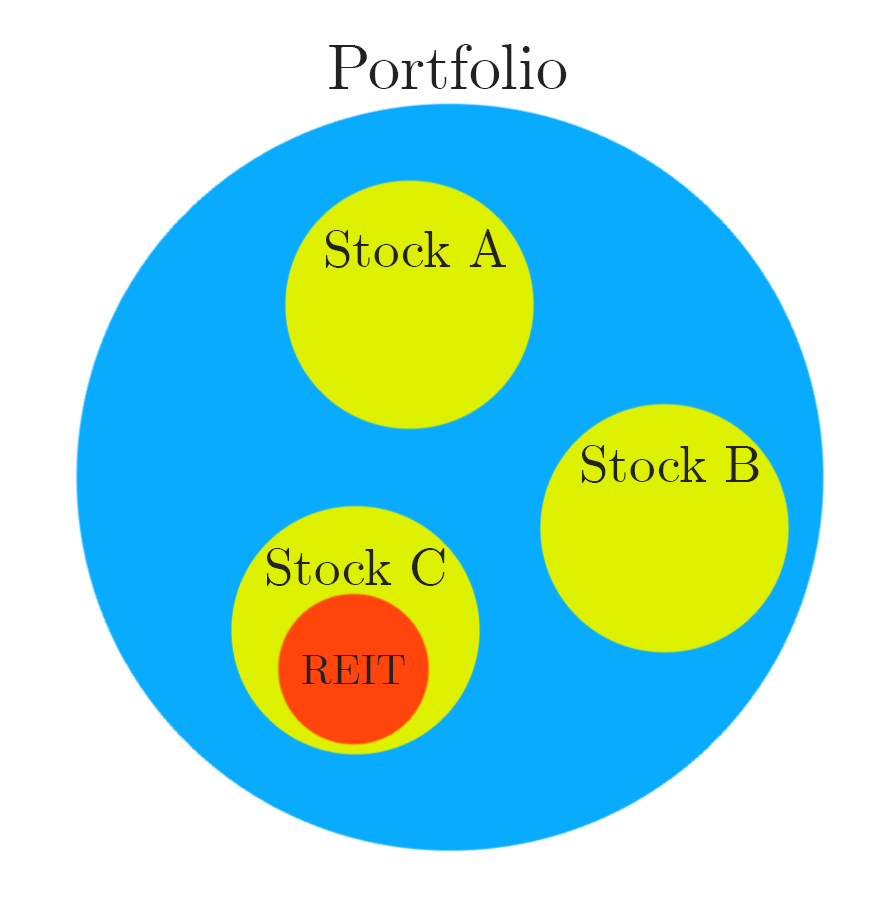
\includegraphics[width=9cm]{Stock_Porfolio_Reit}}
  \caption{Stock vs REIT vs Portfolio}
  \label{fig:Stock_Porfolio_Reit}
  \end{figure}
\subsection{Stock}
A stock also called a share, represents ownership over a company's assets. Each stock is represented in the market by a unique identifier called a ticker. For instance, Apple's ticker is "AAPL". The proportion ownership depends on how many shares are owned out of the total number of shares in the market and stocks of publicily listed companies can be purchased on the stock exchange. Over time, share prices can rise and fall, and owners can receive a share of the company's profits through dividends. The daily movement of the share prices over time will be represented in this paper by the formula:

\begin{itemize}

  \item {Prices: P is the price of a specific stock at a particular time}
  \item {Date: T in this paper is the daily date}
  \item {Ticker: i is the stock ticker for a specific stock}
  
\end{itemize}
\begin{equation*}
  \overrightarrow{P}\textsubscript{i,1:T} =  
  \begin{bmatrix}
    p\textsubscript{i,1} \\
    p\textsubscript{i,2} \\
    \vdots \\
    p\textsubscript{i,T} \\
  \end{bmatrix}
  \in \mathbb{R}_+^{T}
\end{equation*}

\subsection{Real Estate Investment Trusts (REITs)}
A REIT company invests in properties. Typically these companies invest or own a mix of housing, commercial or industrial properties. Buying shares of REITs allow investors to own a share of the real estate that these REITS are managing and indirectly invest their monies in the real estate sector. Of course, each of the 893 REITs are different companies which own a wide range of different properties across the world. In this paper, a REIT is used to refer to the stock of a REIT company. A REIT is a type of stock.

\subsection{Portfolio}
A portfolio is a collection of stocks i.e a portfolio is a combination of more than one stock. For example, the portfolio in Figure ~\ref{fig:Stock_Porfolio_Reit} consists of 10\% of stock A, 11\% of stock B and 9\% of stock C. The relative proportions of each stock in a portfolio can be represented by weights. This paper will represent a portfolio of stocks with the vector and matrix below:
\begin{itemize}

  \item {Weight: W is the percentage value of a ticker in the portfolio.}
  
\end{itemize}

\begin{equation*}
  \overrightarrow{W}\textsubscript{i,1:T}\overrightarrow{P}\textsubscript{i,1:T} = 
  \begin{bmatrix}
    \overrightarrow{W}\textsubscript{1,1:T}\overrightarrow{P}\textsubscript{1,1:T},\;
    \overrightarrow{W}\textsubscript{2,1:T}\overrightarrow{P}\textsubscript{2,1:T},\;
    \ldots,\;
    \overrightarrow{W}\textsubscript{i,1:T}\overrightarrow{P}\textsubscript{2,1:T}
  \end{bmatrix}
\end{equation*}

\begin{equation*}
= 
  \begin{bmatrix}
    w\textsubscript{1,1}\:p\textsubscript{1,1},&
    w\textsubscript{2,1}\:p\textsubscript{2,1},&
    \ldots,&
    w\textsubscript{i,1}\:p\textsubscript{i,1} 
    \\
    w\textsubscript{1,2}\:p\textsubscript{1,2},&
    w\textsubscript{2,2}\:p\textsubscript{2,2},&
    \ldots,&
    w\textsubscript{i,2}\:p\textsubscript{i,2}
    \\
    \vdots&\vdots&\ddots&\vdots
    \\
    w\textsubscript{1,T}\:p\textsubscript{1,T},&
    w\textsubscript{2,T}\:p\textsubscript{2,T},&
    \ldots,&
    w\textsubscript{i,T}\:p\textsubscript{i,T}
  \end{bmatrix}
  \in \mathbb{R}_+^{M x T}
\end{equation*}
\\
As with prices, the weights of each stock ticker can change daily if the value of the portfolio is redistributed. Depending on the weights assigned and what stocks are in the portfolio, the total portfolio value can change rise or fall. The decision of which stocks to select as part of a portfolio and how much of each stock to buy or hold at every point in time is the central idea of portfolio optimisation. This paper seeks to develop an effective model to select stocks and determine these weights.

\subsection{Shorting}
Conventionally, we need to own a certain stock before we can sell it. However, market makers also allow investors to borrow stocks to sell them first, with the contractual obligation for the investor to repurchase the stocks from the market at a later date to return to the market maker. This mechanism of selling first and buying back later is called shorting and is represented by a negative weight. This paper's analysis allows shorting.


\section{Evaluating Investments with Data}
In this subsection, various measures of investment performance and how they are applied in the paper are discussed. It covers the two main schools of thought in investment analysis, technical and fundamental analysis before discussing Alpha formulas.

\subsection{Technical Analysis with Price Volume Data}
Technical analysis is one method of evaluating investments in stocks and identifying prospective stocks to invest in. It focusses primarily on identifying short term trends in price and volume data. Table \ref{table:technical_data} provides the key features required for technical analysis.

\begin{table}[H]
  \centering
  \caption{Daily Price Volume Data for ticker PLD}
  \begin{tabular}{@{} l *{5}{S[table-format=-1.7]} @{}} 
  \toprule
  {Date} & {Open} & {High} & {Low} & {Close} & {Volume}\\ % center-set header entries
  \midrule
  31/08/2023    &  125.36  & 125.91 &  123.89 &  124.2 & 3277600\\
  01/09/2023   &  125.4  & 125.57 &  124.05 &  124.59 & 1591000\\
  05/09/2023 &  125.36  & 125.91 &  123.89 &  122.05 & 2854100\\
  \bottomrule
  \end{tabular}
  \label{table:technical_data}
\end{table}

\begin{itemize}

  \item {Open: The price of the stock at the start of a trading day}
  \item {High: The highest price of the stock in a trading day}
  \item {Low: The lowest price of the stock in a trading day}
  \item {Close: The price of the stock when the market closes for the day}
  \item {Volume: The total number of shares traded throughout the day}
  
\end{itemize}
The features Open, High, Low and Close are derived from the Price of a stock at different points in the day and trends of these features can indicate future movements, while volume signals the strength of a price trend.

\subsubsection{Profit and Loss (PnL)}
Profits from the purchase of a single stock arises when the selling price of the stock is greater than the original purchase price. However, if the share price falls below the original purchase price then a loss is incurred. Profit or Loss is given by the formula: 
\begin{equation*}
  Profit/Loss = Current Price \times Quantity - Purchase Price \times Quantity
\end{equation*}

\pgfplotstableread{2.pnlDay1.dat}\datatable
\pgfplotstableread{2.pnlDay3.dat}\datatable
\begin{figure}[H]
  \centering
  \centerline{Prices and Profits from Stock A, Purchasing on Different Days}
  \par\medskip
  \begin{subfigure}{.475\linewidth}
    \centering
  \begin{tikzpicture}
  \begin{axis}[
    small,
    xlabel=Day,
    ylabel=\$,
    legend style={at={(0.5,-0.3)},anchor=north},
    smooth,
    ]
  \addplot[mark=*,blue] table [x=Day, y=$SharePrice$]{2.pnlDay1.dat};
  \addlegendentry{$SharePrice$ series}
  \addplot[mark=x,green] table [x=Day, y=$Profit$]{2.pnlDay1.dat};
  \addlegendentry{$Profit$ series}
  \end{axis}
  \end{tikzpicture}
  \caption{Day 1 Purchase}
  \label{graph: prices_and_profits}
\end{subfigure}%
\hfill%
\begin{subfigure}{.475\linewidth}
  \centering
  \begin{tikzpicture}
    \begin{axis}[
      small,
      xlabel=Day,
      ylabel=\$,
      legend style={at={(0.5,-0.3)},anchor=north},
      smooth,
      ]
    \addplot[mark=*,blue] table [x=Day, y=$SharePrice$]{2.pnlDay3.dat};
    \addlegendentry{$SharePrice$ series}
    \addplot[mark=x,red] table [x=Day, y=$Profit$]{2.pnlDay3.dat};
    \addlegendentry{$Profit$ series}
    \end{axis}
    \end{tikzpicture}
    \caption{Day 3 Purchase}
    \label{graph: prices_and_profits2}
  \end{subfigure}
  \caption{}
  \label{figure: prices_and_profits_main}
\end{figure}

It's important to note that profits or losses are only realised when the closing transaction is made i.e. when the stock is sold. Figure \ref{figure: prices_and_profits_main} illustrates that buying the same stock on day 1 versus day 3 can have vastly different results. \\

When a stock is shorted, a rise in price will result in a loss because it becomes more expensive for the investor to repurchase the share. Hence, for shorting the Profit or Loss formula is negated:
\begin{equation*}
  Profit/Loss = -(Current Price \times Quantity - Purchase Price \times Quantity)
\end{equation*}


\subsubsection{Risk and Volatility} \label{Risk and Volatility}
Volatility is a statistical measure of how varied share price and returns on an investment are over a period of time. It is a proxy of the risk of an investment, the likelihood of an investment performing worse than expected. \\
\begin{figure}[H]
  \centering
  \centerline{Prices and Profits from Stock A, Purchasing on Different Days}
  \par\medskip
  \begin{subfigure}{.475\linewidth}
    \centering
    \pgfmathdeclarefunction{gauss}{2}{%
            \pgfmathparse{1/(#2*sqrt(2*pi))*exp(-((x-#1)^2)/(2*#2^2))}%
        }

        \begin{tikzpicture}

        \def\startx{0}    % lower end of domain
        \def\endx{7}       % upper end of domain
        \def\camean{3}  % mean of left side distribution
        \def\casigma{1}  % sigma for left side distribution
        \def\cbmean{3.0}   % mean for right side distribution
        \def\cbsigma{0.5}  % sigma for right side distribution
        \def\verticala{0.7} % x vale for first delimiter
        \def\verticalb{1.3} % x value for second delimited

        \begin{axis}[
        domain=\startx:\endx,
        samples=101,
        ymax=1.2,
        enlargelimits=false,
        axis x line=middle,
        axis y line=middle,
        xtick={0,3},
        xticklabels={0,3},
        ytick={\empty},
        xlabel={$Price$},
        ylabel={$Frequency$},
        height=5cm,
        width=7cm
        ]
        % Draw distributions
        \addplot [name path=a,thin, smooth] {gauss(\camean,\casigma)};
        \addplot [name path=b,thin, smooth] {gauss(\cbmean,\cbsigma)};%    
        % Draw vertical lines:
        %\draw [gray, semithick] (\verticala,0) -- (\verticala,0.4);
        %\draw [gray, semithick] (\verticalb,0) -- (\verticalb,0.4);
        % create path for x axis:
        \path[name path=axis] (axis cs:\startx,0) -- (axis cs:\endx,0);
        % generate fills:
        %\addplot[darkgray]  fill between[of=a and axis,soft clip={domain=\verticala:\verticalb}]; % 
        %\addplot[pattern=north east lines]  fill between[of=b and a,
        %soft clip={(\verticala,0) rectangle (\verticalb,0.5)}
        %]; 
        % place the labels for each distribution
        \node (a) at (3,0.9) {Stock A};
        \node (b) at (5,0.4) {Stock B};

        \end{axis}

        \end{tikzpicture}
        \caption{Price Risk}
        \label{graph: risk_price}
      \end{subfigure}%
      \hfill%
      \begin{subfigure}{.475\linewidth}
      \centering
      \pgfmathdeclarefunction{gauss}{2}{%
            \pgfmathparse{1/(#2*sqrt(2*pi))*exp(-((x-#1)^2)/(2*#2^2))}%
        }

        \begin{tikzpicture}

        \def\startx{0}    % lower end of domain
        \def\endx{7}       % upper end of domain
        \def\camean{3}  % mean of left side distribution
        \def\casigma{1}  % sigma for left side distribution
        \def\cbmean{2.0}   % mean for right side distribution
        \def\cbsigma{0.5}  % sigma for right side distribution
        \def\verticala{0.7} % x vale for first delimiter
        \def\verticalb{1.3} % x value for second delimited

        \begin{axis}[
        domain=\startx:\endx,
        samples=101,
        ymax=1.2,
        enlargelimits=false,
        axis x line=middle,
        axis y line=middle,
        xtick={0,3},
        xticklabels={0,3},
        ytick={\empty},
        xlabel={$Return$},
        ylabel={$Frequency$},
        height=5cm,
        width=7cm
        ]
        % Draw distributions
        \addplot [name path=a,thin, smooth] {gauss(\camean,\casigma)};
        \addplot [name path=b,thin, smooth] {gauss(\cbmean,\cbsigma)};%    
        % Draw vertical lines:
        \draw [gray, semithick] (2,0) -- (2,1);
        \draw [gray, semithick] (3,0) -- (3,0.7);
        % create path for x axis:
        \path[name path=axis] (axis cs:\startx,0) -- (axis cs:\endx,0);
        % generate fills:
        %\addplot[darkgray]  fill between[of=a and axis,soft clip={domain=\verticala:\verticalb}]; % 
        %\addplot[pattern=north east lines]  fill between[of=b and a,
        %soft clip={(\verticala,0) rectangle (\verticalb,0.5)}
        %]; 
        % place the labels for each distribution
        \node (a) at (3,0.9) {Stock A};
        \node (b) at (4,0.5) {Stock B};

        \end{axis}
        
        \end{tikzpicture}
        \caption{Return Risk}
    \label{graph: risk_returns}
  \end{subfigure}
  \caption{}
  \label{figure: risk_volatility_main}
\end{figure}

Figure \ref{graph: risk_price} shows the distribution of prices of Stocks A and B over a period of time. Stock A has a lower standard deviation $\sigma_A$ than Stock B $\sigma_B$, lower volatility and lower price risk.  The returns on both stocks can also be plotted on a similiar distribution as shown in Figure \ref{graph: risk_returns}. Because this paper seeks to minimise risk, the variance of prices and returns need to be considered.

\subsubsection{Sharpe Ratio}
Deciding between stocks or portfolios with different expected returns and risk like in Figure \ref{graph: risk_returns} where Stock B has higher returns but also higher risk than Stock A, requires a formula that evaluates these two measures together. The sharpe ratio combines both measures of profit/loss and risk into a single formula as follows:
\begin{equation*}
  Sharpe Ratio = \frac{R\textsubscript{p}-R\textsubscript{f}}{\sigma\textsubscript{p}}
\end{equation*}
\begin{itemize}
  \item {$R_p$: The annualised return of portfolio}
  \item {$R_f$: The risk free rate}
  \item {$\sigma_p$: The standard deviation of portfolio return}
\end{itemize}
The risk free rate $R_f$ is the return from a zero risk investment such as government bonds. Hence $R_p - R_f$ gives us the excess returns of the portfolio investment compared to a zero risk investment. $\sigma_p$ measures volatility as covered in section \ref{Risk and Volatility}. 
\\

In this paper, the sharpe ratio is used as the overall measure of performance of the portfolio optimisation models and is incorporated in the various objective functions. 
\subsection{Fundamental Analysis with Financial Statements}
Fundamental analysis is a second method of investment analysis that is widely used by finance practitioners but less often applied by Machine Learning researchers. It involves examining the assets and incomes of the companies behind the different stock tickers by looking at their financial statements to evaluate the intrinsic value of a stock. 
\begin{figure}[H]
  \centerline{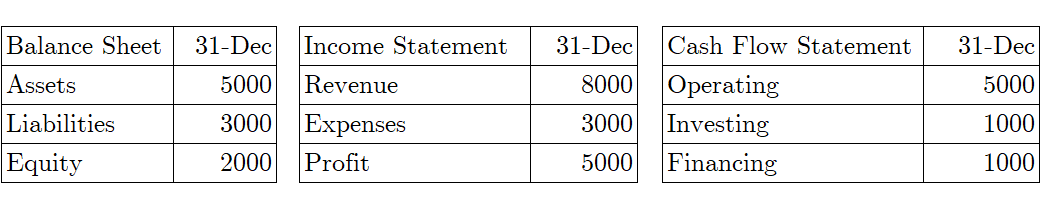
\includegraphics[width=17cm]{financial_statements}}
  \caption{Highly Abbreviated 3 Main Statements}
  \label{fig:financial statements}
\end{figure}
Every quarter, every company with a stock ticker will publish its financial statements which consists of the Balance Sheet, Income Statement and Cash Flow Statement. Figure \ref{fig:financial statements} is a highly abbreviated example, the real financial statements breaks down each category into hundreds of subcategories which can be used as features for Machine Learning.\\

The predictive value of each statement is as follows:
\begin{itemize}
  \item {Income Statement: Profitability of the company's business and the rate of growth of its value}
  \item {Balance Sheet: The asset value and financial stability of the company }
  \item {Cash Flow Statement: How cash is generated by the company}
\end{itemize}

Incorporating both technical and fundamental data into machine learning models can provide a more holistic picture to the analysis and better inform these models with an extended set of short, medium and long term features.

\subsection{Alpha Formulas}
According to quant researcher Tulchinsky (2019), an Alpha is a formula that determines how much capital to allocate to each stock every day. A good alpha allocates capital in a way that results in a high sharpe ratio for the entire portfolio.\\

Here are two examples of alpha formulas used in real-life trading from a paper by Kakushadze (2016): \\

Alpha 1: $(((high * low)^{0.5}) - vwap)$\\

Alpha 2: $((0.25 < (((delay(close, 20) - delay(close, 10)) / 10) - ((delay(close, 10) - close) / 10))) ?
(-1 * 1) : (((((delay(close, 20) - delay(close, 10)) / 10) - ((delay(close, 10) - close) / 10)) < 0) ? 1 :
((-1 * 1) * (close - delay(close, 1)))))$ \\

The first formula Alpha 1 is relatively simple while Alpha 2 is complex. \\

Figure \ref{fig:alpha table} demonstrates how Alpha 1 is applied to portfolio allocation in a stock portfolio of 6 tickers. Every day, each stock ticker will have its own Alpha value in the first green column of Figure, derived by passing the required features as inputs to the alpha formula (e.g. in this case, Alpha 1 requires, High, Low and Volume Weighted Average Price (Vwap)). \\

\begin{figure}[H]
  \centerline{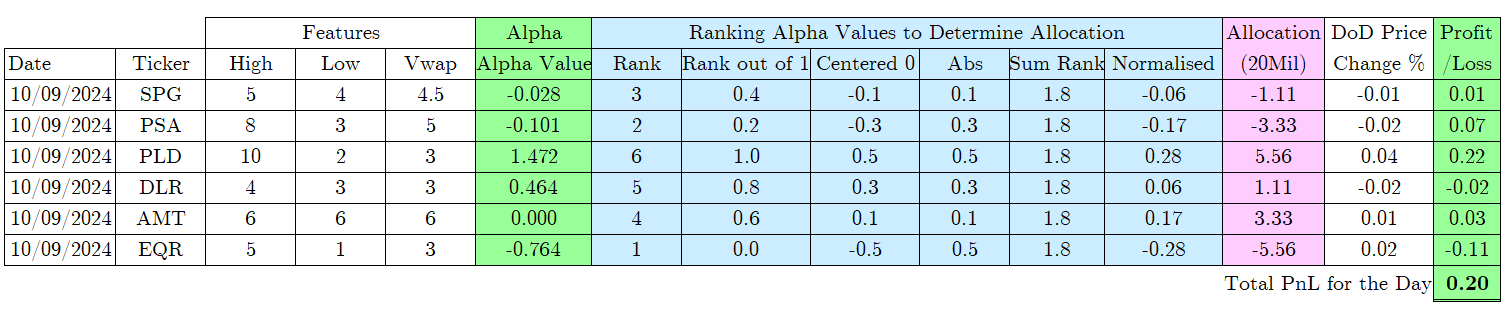
\includegraphics[width=20cm]{alpha_table}}
  \caption{Application of Alpha 1 to Porfolio Allocation}
  \label{fig:alpha table}
\end{figure}

In the blue section of \ref{fig:alpha table}, the Alpha values are then ranked, centered and normalised to determine the relative proportion of the portfolio to allocate to each stock ticker. In a portfolio of 6 tickers, the largest 3 ranks will be bought and the lowest 3 ranks will be shorted to differing degrees. \\

In the pink column, 20 million in capital is allocated by multiplying the total capital of 20 million by the normalised rank. The allocation amount mulitplied by the day-on-day percentage price change (Dod Price Change \%) for each ticker will then give us the Profit/Loss for each stock ticker for the day. The (Dod Price Change \%) formula is as follows:
\begin{equation*}
  (Dod\:Price\:Change\:\%) = \frac{Pave\textsubscript{t+1}-Pave\textsubscript{t}}{|Pave\textsubscript{t}|}
\end{equation*}

\begin{itemize}
  \item {$Pave_{t+1}$: Average of Tommorrow's Open and Close Price}
  \item {$Pave_{t}$: Average of Today's Open and Close Price}
\end{itemize}

The total sum of the Profit/Loss for every ticker is the PnL from the day's investment as all positions are closed and the capital is reallocated the following day. \\

This paper seeks to apply Alpha formulas to allocate REIT portfolios, and go further by developing a Genetic Algorithm inspired by Charles Darwin's theory of evolution to search for strong Alphas to Optimise Real Estate Portfolios. 

\subsection{Other Methods of Analyses}
Sentiment Analysis: Given that share prices in the short run are largely driven by investor sentiment, some researchers have employed Natural Language Processing (NLP) techniques to process trade forum discussions and financial news for trade decision making resulting in good sharpe ratios (Alexandria, 2023). \\

Macro-economic Analysis: Considering various measures of the wider economic environment such as GDP growth rates, unemployment rates, inflation and interest rates are important as well because these are strong factors that can influence the overall market performance. It suggests the broader market direction.

\begin{landscape}
\titlespacing{\chapter}{53pt}{-70pt}{1cm}% <-- spacing of title bar
\chapter{Literature Review of Portfolio Optimisation Techniques}

\def\fillandplacepagenumber{%
 \par\pagestyle{empty}%
 \vbox to 0pt{\vss}\vfill
 \vbox to 0pt{\baselineskip0pt
   \hbox to\linewidth{\hss}%
   \baselineskip\footskip
   \hbox to\linewidth{%
     \hfil\thepage\hfil}\vss}}


  
  \titlespacing{\section}{0pt}{-150pt}{0cm}% <-- spacing of title bar
  \section{Comparison of Traditional and Machine Learning Techniques}
  \begin{table}[H]
    \begin{adjustwidth}{-1.25cm}{-1.25cm}
    \begin{tabular}{|p{2.6cm}|p{2.7cm}|p{2.7cm}|p{3.5cm}|p{5cm}|p{5cm}|p{4cm}|}
    \hline
    \textbf{Methods} & \textbf{Data Inputs} & \textbf{Objectives} & \textbf{Scope for REITs} & \textbf{Strengths} & \textbf{Weaknesses} & \textbf{References}  
    \\ \hline Autoregressive Integrated Moving Average (ARIMA) & Daily Price-Volume Data & Stock Price Prediction and Clustering & Stock Price Prediction & +Suitable for short-term time-series analysis \par+ Widely used in the field of finance for prediction \par+ More explanable than complex ML models & \par-Unsatisfactory for long term prediction \par-Higher RMSE than ML models   & (Ariyo et.al., 2014),\par (Habbab \& Kampouridis, 2022),\par   (Obthong et. al., 2020)        
    \\ \hline Generalised AutoRegressive Conditional Heteroskedasticity (GARCH) & Daily Commodities Price-Volume data & Stock Volatility Prediction & Stock Volatility Prediction & +Outperforms ARIMA for price prediction and volatility forcasting & - Model assumes volatility can be predicted based on past returns, but volatility in reality is very unpredicatable & (Fiszeder \& Chung, 2020),   (Lama et. al., 2015), (Yuan et. al, 2017           
    \\ \hline Multiple Linear Regression (MLR) & Daily Price-Volume Data & Stock Price Prediction & Stock Price Prediction & +Relatively low RMSE error for stock price prediction \par+ Relatively easy to implement & - Only considers input features and not historical price data  & (Obthong et. al., 2020), (Shakhla et. al., 2023)
    \\ \hline 
    \end{tabular}
  \end{adjustwidth}
  \end{table}
  \section{Comparison of Traditional and Machine Learning Techniques (Continued)}
  \begin{table}[H]
    \begin{adjustwidth}{-1.25cm}{-1.25cm}
    \begin{tabular}{|p{2.6cm}|p{2.7cm}|p{2.7cm}|p{3.5cm}|p{5cm}|p{5cm}|p{4cm}|}
    \hline
    \textbf{Methods} & \textbf{Data Inputs} & \textbf{Objectives} & \textbf{Scope for REITs} & \textbf{Strengths} & \textbf{Weaknesses} & \textbf{References}  
    \\ \hline\rowcolor[gray]{.8}Recurrent Neural Networks (RNN) & Daily Price-Volume Data & Stock Price Prediction & & +Relatively low RMSE error for stock price prediction\par + Remembers historical stock prices & - Susceptible to vanishing and exploding gradient problem & (Dey et. al., 2021) 
    \\ \hline Long-Short Term Memory (LSTM) & Daily Price-Volume Data & Stock Price Prediction & Stock Price Prediction & + One of the lowest RMSE error for financial time series prediction \par+ Remembers historical stock prices which are good indicators of future prices \par+ Solves the vanishing and exploding gradient problem & - Mixed results when predicting REIT stock prices & (Axelsson \& Song, 2023),   (Habbab \& Kampouridis, 2022), (Obthong et. al., 2020) 
    \\ \hline\rowcolor[gray]{.8} Random Forest (RF) & Daily Price-Volume Data, Fundamental Data & Stock Price Prediction & & + One of the few papers to incorporate fundamental data into machines learning models & - Relatively low sharpe ratio compared to market indexes & (Cao, 2021), (Huang et. al., 2021)  
    \\ \hline Genetic Algorithms & Daily Price-Volume Data & Stock Price Prediction and Clustering & & + Suitable for problems with a large search space \par+ Works well with large time-series data & & (Obthong et. al., 2020) 
    \\ \hline
    \end{tabular}
  \end{adjustwidth}
  \end{table}
  %\fillandplacepagenumber



  
\end{landscape}



\subsection{Predictive Accuracy}
A recent paper aimed at predicting REIT share prices through 5 machine learning algorithms and 3 traditional benchmarks, which includes many of the methods in Section 3.2 above, found that machine learning models (MLR, LSTM) appear more accurate than traditional benchmarks (ARIMA). The algorithms were trained solely on daily price data, and Figure \ref{fig:lit_review_rmse} shows the RMSE results for out-of sample predictions over different time periods (30, 60, 90, 120 and 150 days).


\begin{figure}[H]
  \centerline{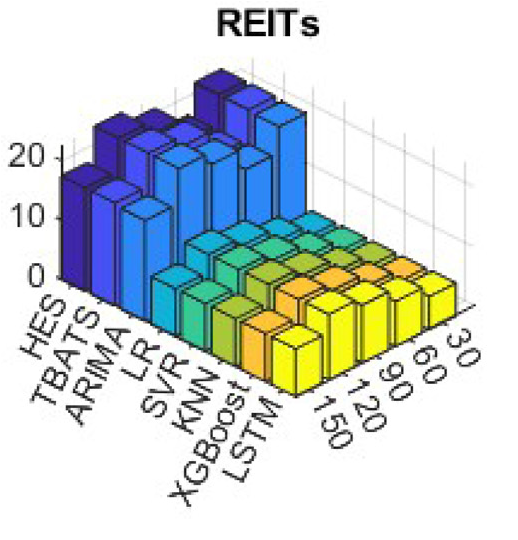
\includegraphics[width=5cm]{lit_review_reit_rmse}}
  \caption{RMSE results for REITs using various ML Models (Source: Habbab \& Kampouridis, 2024)}
  \label{fig:lit_review_rmse}
\end{figure}


\subsection{Gaps in Past Research to be Addressed}
From the literature review in Section 3.3, it appears that there are the following gaps that can be further explored in this paper:
\begin{enumerate}

  \item {From the "Data Inputs" column, it appears most papers use price-volume (technical) data without fundamental data to make predictions.}
  \item {From the "Objectives" column, most papers are focussed on predicting stock prices and rarely address portfolio allocation or optimisation (i.e. to use these predictions to inform buy/sell decision of each stock in a portfolio or to find the optimal weights of each stock in a portfolio to maximise the sharpe ratio).}
  \item {There are no papers about searching for Alphas for REIT portfolios}
  \item {Even though genetic algorithms have been used to predict stock prices, there appears to be an opportunity to apply it to the search of outperforming REIT Alphas.}
  
\end{enumerate}






\titleformat{\chapter}[block]
  {\normalfont\huge\bfseries}{\thechapter.}{1em}{\Huge\centering}
\titlespacing*{\chapter}{0pt}{230pt}{0pt}
\setcounter{chapter}{1}
\renewcommand{\thechapter}{\Roman{chapter}}
\chapter{Innovation}

\titleformat{\chapter}[display]{\Large}{\centering
  \MakeUppercase{\chaptername}\quad{\Huge\thechapter}}{0pt}{\titlerule[.5pt]\vspace{10pt}\centering
  \MakeUppercase}[\vspace{10pt}{\titlerule[.5pt]}]% <-- spacing of title bar
\titlespacing{\chapter}{0pt}{-80pt}{1cm}% <-- spacing of title bar
\renewcommand{\thechapter}{\arabic{chapter}}
\setcounter{chapter}{3}
\pagenumbering{arabic}
\chapter{Datasets}
\section{Extended Fundamental Data Features}
While many papers have obtained price-volume data from Yahoo Finance's API (yfinance), this data only contains 10 or so price-volume indicators listed in Appendix A. This paper goes further by obtaining a comprehensive list of 161 fundamental features from FinancialModelingPrep's (FMP) API\footnote{Although the datasource is proprietory and the author does not have permission to distribute the raw data, it can be easily purchased for a small fee at https://site.financialmodelingprep.com/.}, listed in Appendix B. 

\tikzstyle{every node}=[font=\large]
\begin{figure}[H]
  \centering
  \begin{tikzpicture}
    \pie[pos={0,0},radius=3,sum=auto,text=legend]{10/Technical, 161/Fundamental}
    \end{tikzpicture}
    \caption{Count of Fundamental vs Technical Features}
    \label{fund_tec_pie}
  \end{figure}

  A script was written to combine the data from various api endpoints and backfill any missing values. Because price-volume data is available daily while fundamental data is generally available quarterly, a function is written to backfill the fundamental data such that daily numbers are available.



\section{Feature Exploration with Decision Trees}
Running a 25 layer Decision Tree on all 171 features reveals the strongest predictors for the next day's closing price. The top 4 layers are in Figure \ref{fig:decision_tree_features}:


\begin{figure}[H]
  \centerline{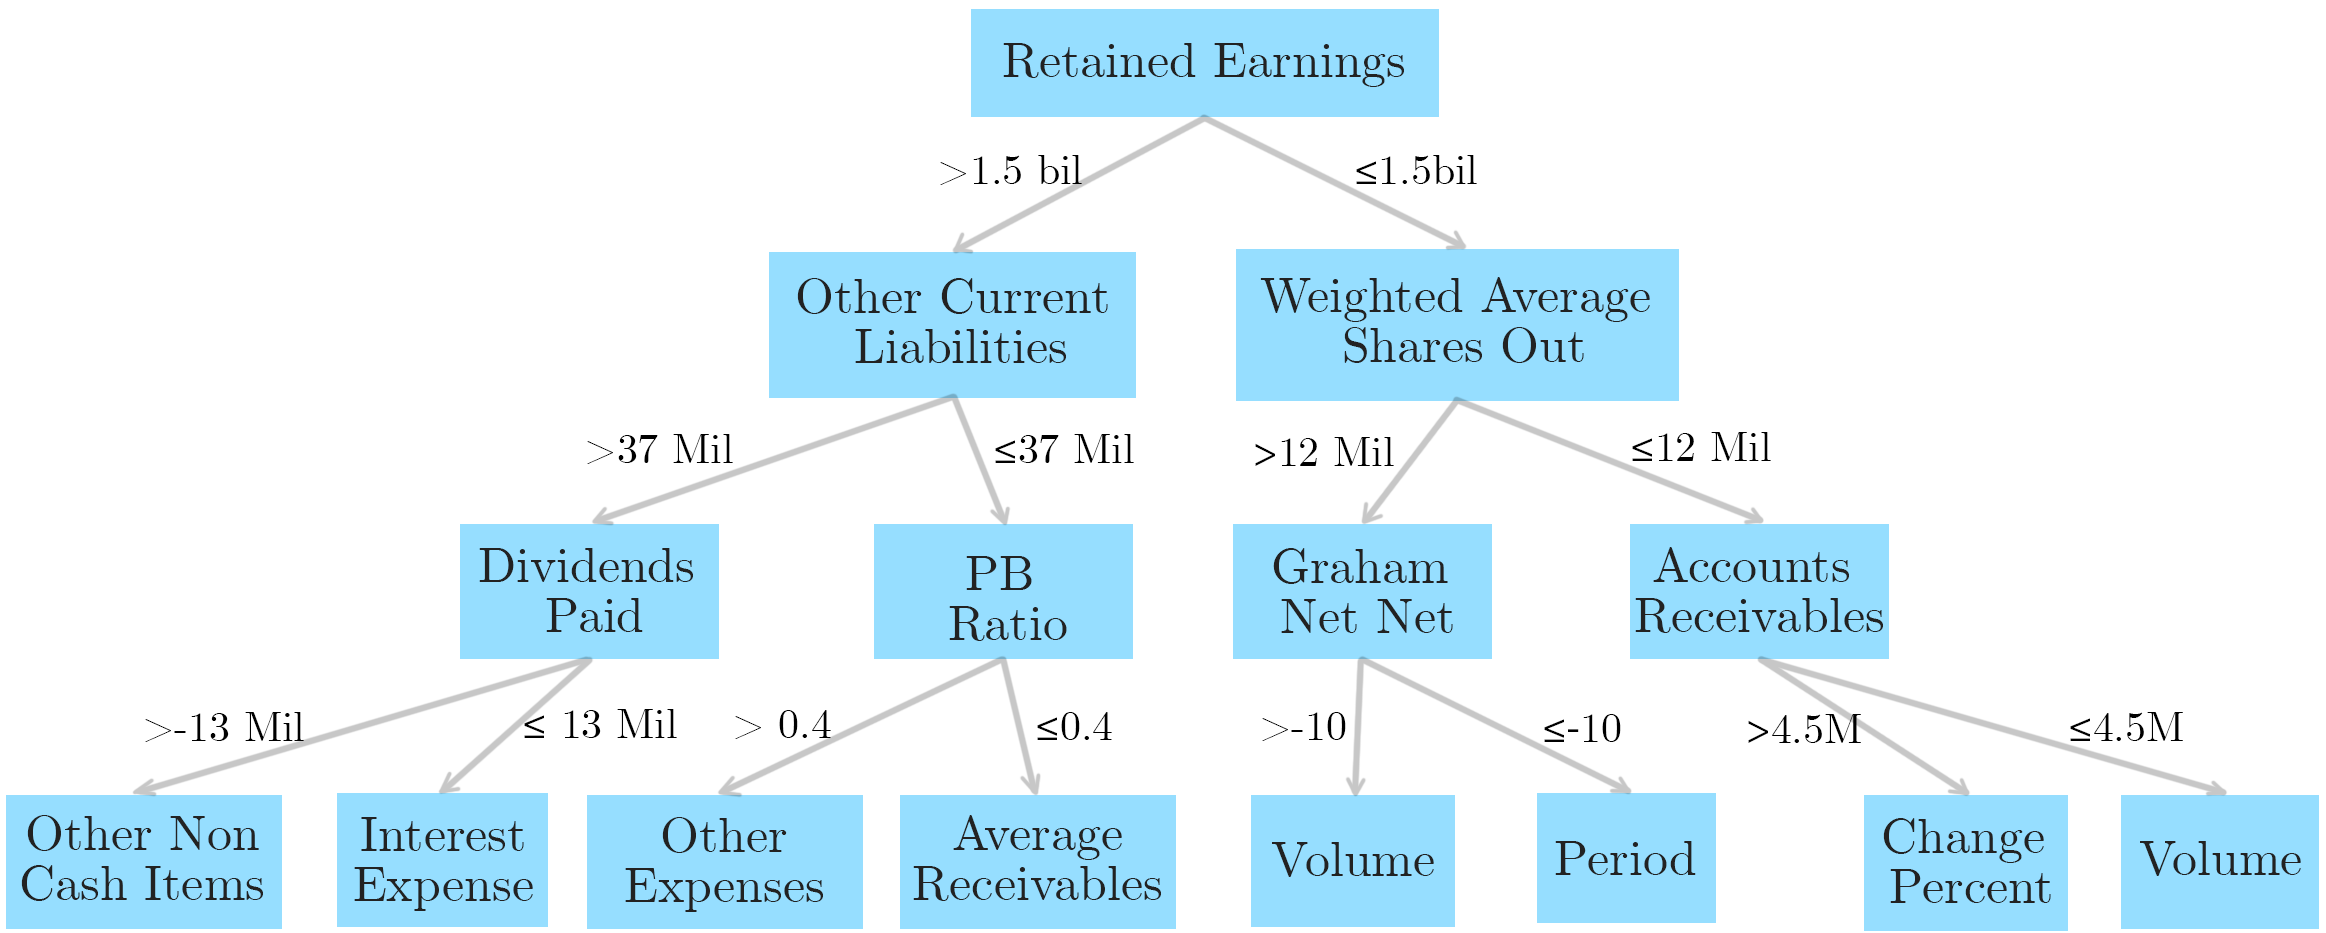
\includegraphics[width=16cm]{feature_decision_tree}}
  \caption{Top 4 Layers of Decision Tree To Predict T+1 Close}
  \label{fig:decision_tree_features}
\end{figure}

Figure \ref{fig:decision_tree_horizontal_graph} also shows the weights of the top 10 features in the Decision Tree. From both figures, it appears many of the balance sheet, income and cash flow statement features are indeed strong predictors of share price, coupled with technical features like Volume and Percentage Change in Share Price. 

\begin{figure}[H]
  \centerline{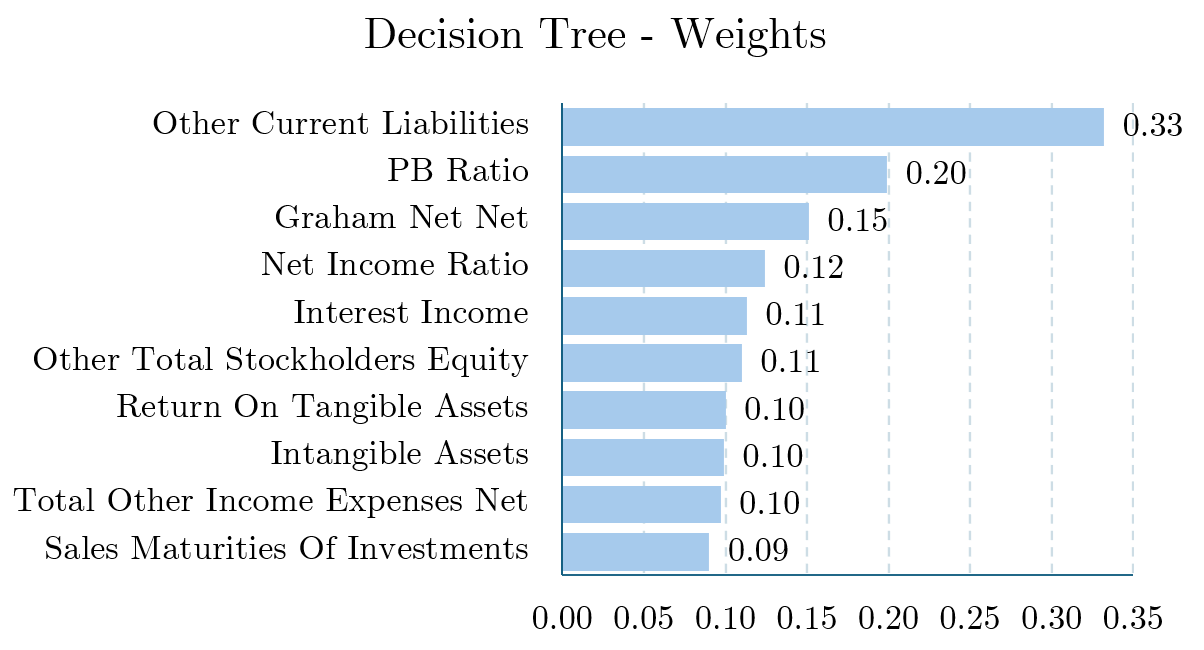
\includegraphics[width=10.5cm]{decision_tree_horizontal_graph}}
  \caption{Top 10 Feature Weights from Decision Tree}
  \label{fig:decision_tree_horizontal_graph}
\end{figure}

\section{Feature Selection}
From the decision tree, it also appears that many of the top features can be encapsulated by other features. For example, Other Current Liabilities is a component of Total Current Liabilities, Expenses are part of Net Income and Cash Items are a part of Cash From Activities. Given that the tree was generated from only one stock ticker, to make the feature selection generalisable to all 150 tickers, the results are contextualised with financial knowledge to derive the final 22 Selected Features presented in Figure \ref{fig:selected_features}. The financial significance of each feature is explained in the column "Domain Importance".
\begin{figure}[H]
  \centerline{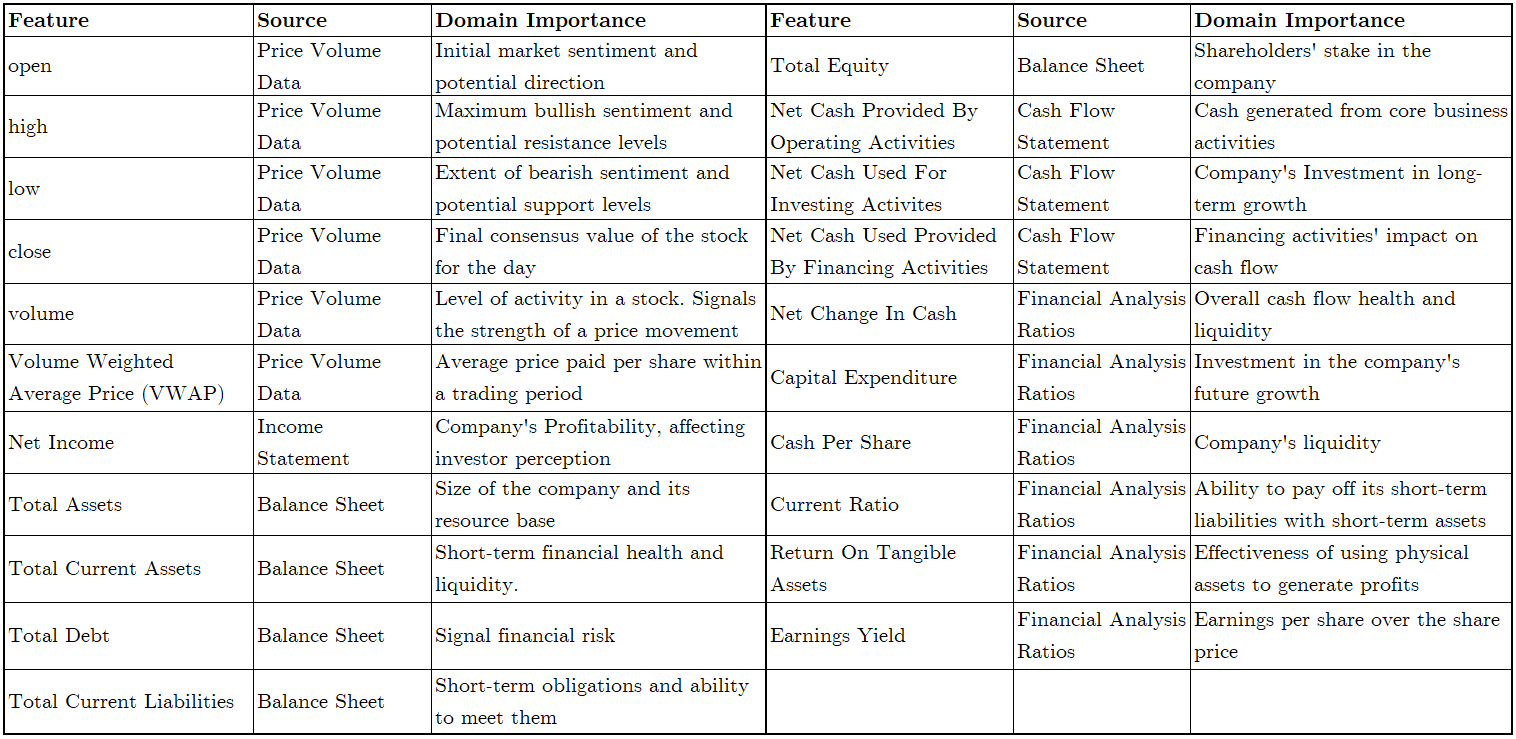
\includegraphics[width=20cm]{selected_features}}
  \caption{22 Input Features Selected for Models}
  \label{fig:selected_features}
\end{figure}
In the preprocessing step, up to 20 years of historical data with these 22 features are retrieved for 150 stock tickers, and appended to a dictionary which stores all the required data for each ticker.

\iffalse

\begin{figure}[H]
  \centering
  \begin{tikzpicture}[x={(.01,0)}]
  \foreach  \l/\x/\c[count=\y] in {Net Income Ratio/0.12/NetIncomeRatio, 
  Graham Net Net/0.15/GrahamNetNet, 
  Pb Ratio/0.20/PbRatio, 
  Other Current Liabilities/0.33/OtherCurrentLiabilities}
  {\node[left] at (0,\y) {\l};
  %\fill[\c] (0,\y-.4) rectangle (\x,\y+.4);
  \node[right] at (\x, \y) {\x};}
  \draw (0,0) -- (0.5,0);
  \foreach \x in {0.05, 0.10, ..., 0.6}
  {\draw (\x,.2) -- (\x,0) node[below] {\x};}
  \draw (0,0) -- (0,4.5);
  \end{tikzpicture}
\end{figure}





% commented out latex tree, use photoshop instead
\begin{tikzpicture}[
  grow=down,
  level 1/.style={sibling distance=3.5cm,level distance=2cm},
  level 2/.style={sibling distance=3.5cm, level distance=2cm},
  edge from parent/.style={very thick,draw=blue!40!black!60,
      shorten >=5pt, shorten <=5pt},
  edge from parent path={(\tikzparentnode.south) -- (\tikzchildnode.north)},
  kant/.style={text width=2cm, text centered, sloped},
  every node/.style={text ragged, inner sep=2mm},
  punkt/.style={rectangle, rounded corners, shade, top color=white,
  bottom color=blue!50!black!20, draw=blue!40!black!60, very
  thick }
  ]

\node[punkt, text width=5.5em] {Country~\A}
  %Lower part lv1
  child {
      node[punkt, text width=6em] {Country~\A}
      edge from parent
          node[kant, below, pos=.6] {Unchanged parity}
  }
  %Upper part, lv1
  child {
      node[punkt, text width=6em] {Country~\A}
      %child 1
      child {
          node[punkt, text width=6em] {Country~\A}
          edge from parent
              node[below, kant,  pos=.6] {Unchanged parity}
      }
      %child 2
      child {
          node[punkt, text width=6em] {Country~\A}
          edge from parent
              node[kant, above] {Devalues}}
          edge from parent{
              node[kant, above] {Devalues}}
  };
\end{tikzpicture}
\fi


\chapter{Methodology}
This paper takes two approaches to portfolio optimisation. 1) Optimisation with Machine Learning and 2) Alpha Tree Search using Genetic Algorithms.
\begin{figure}[H]
\centerline{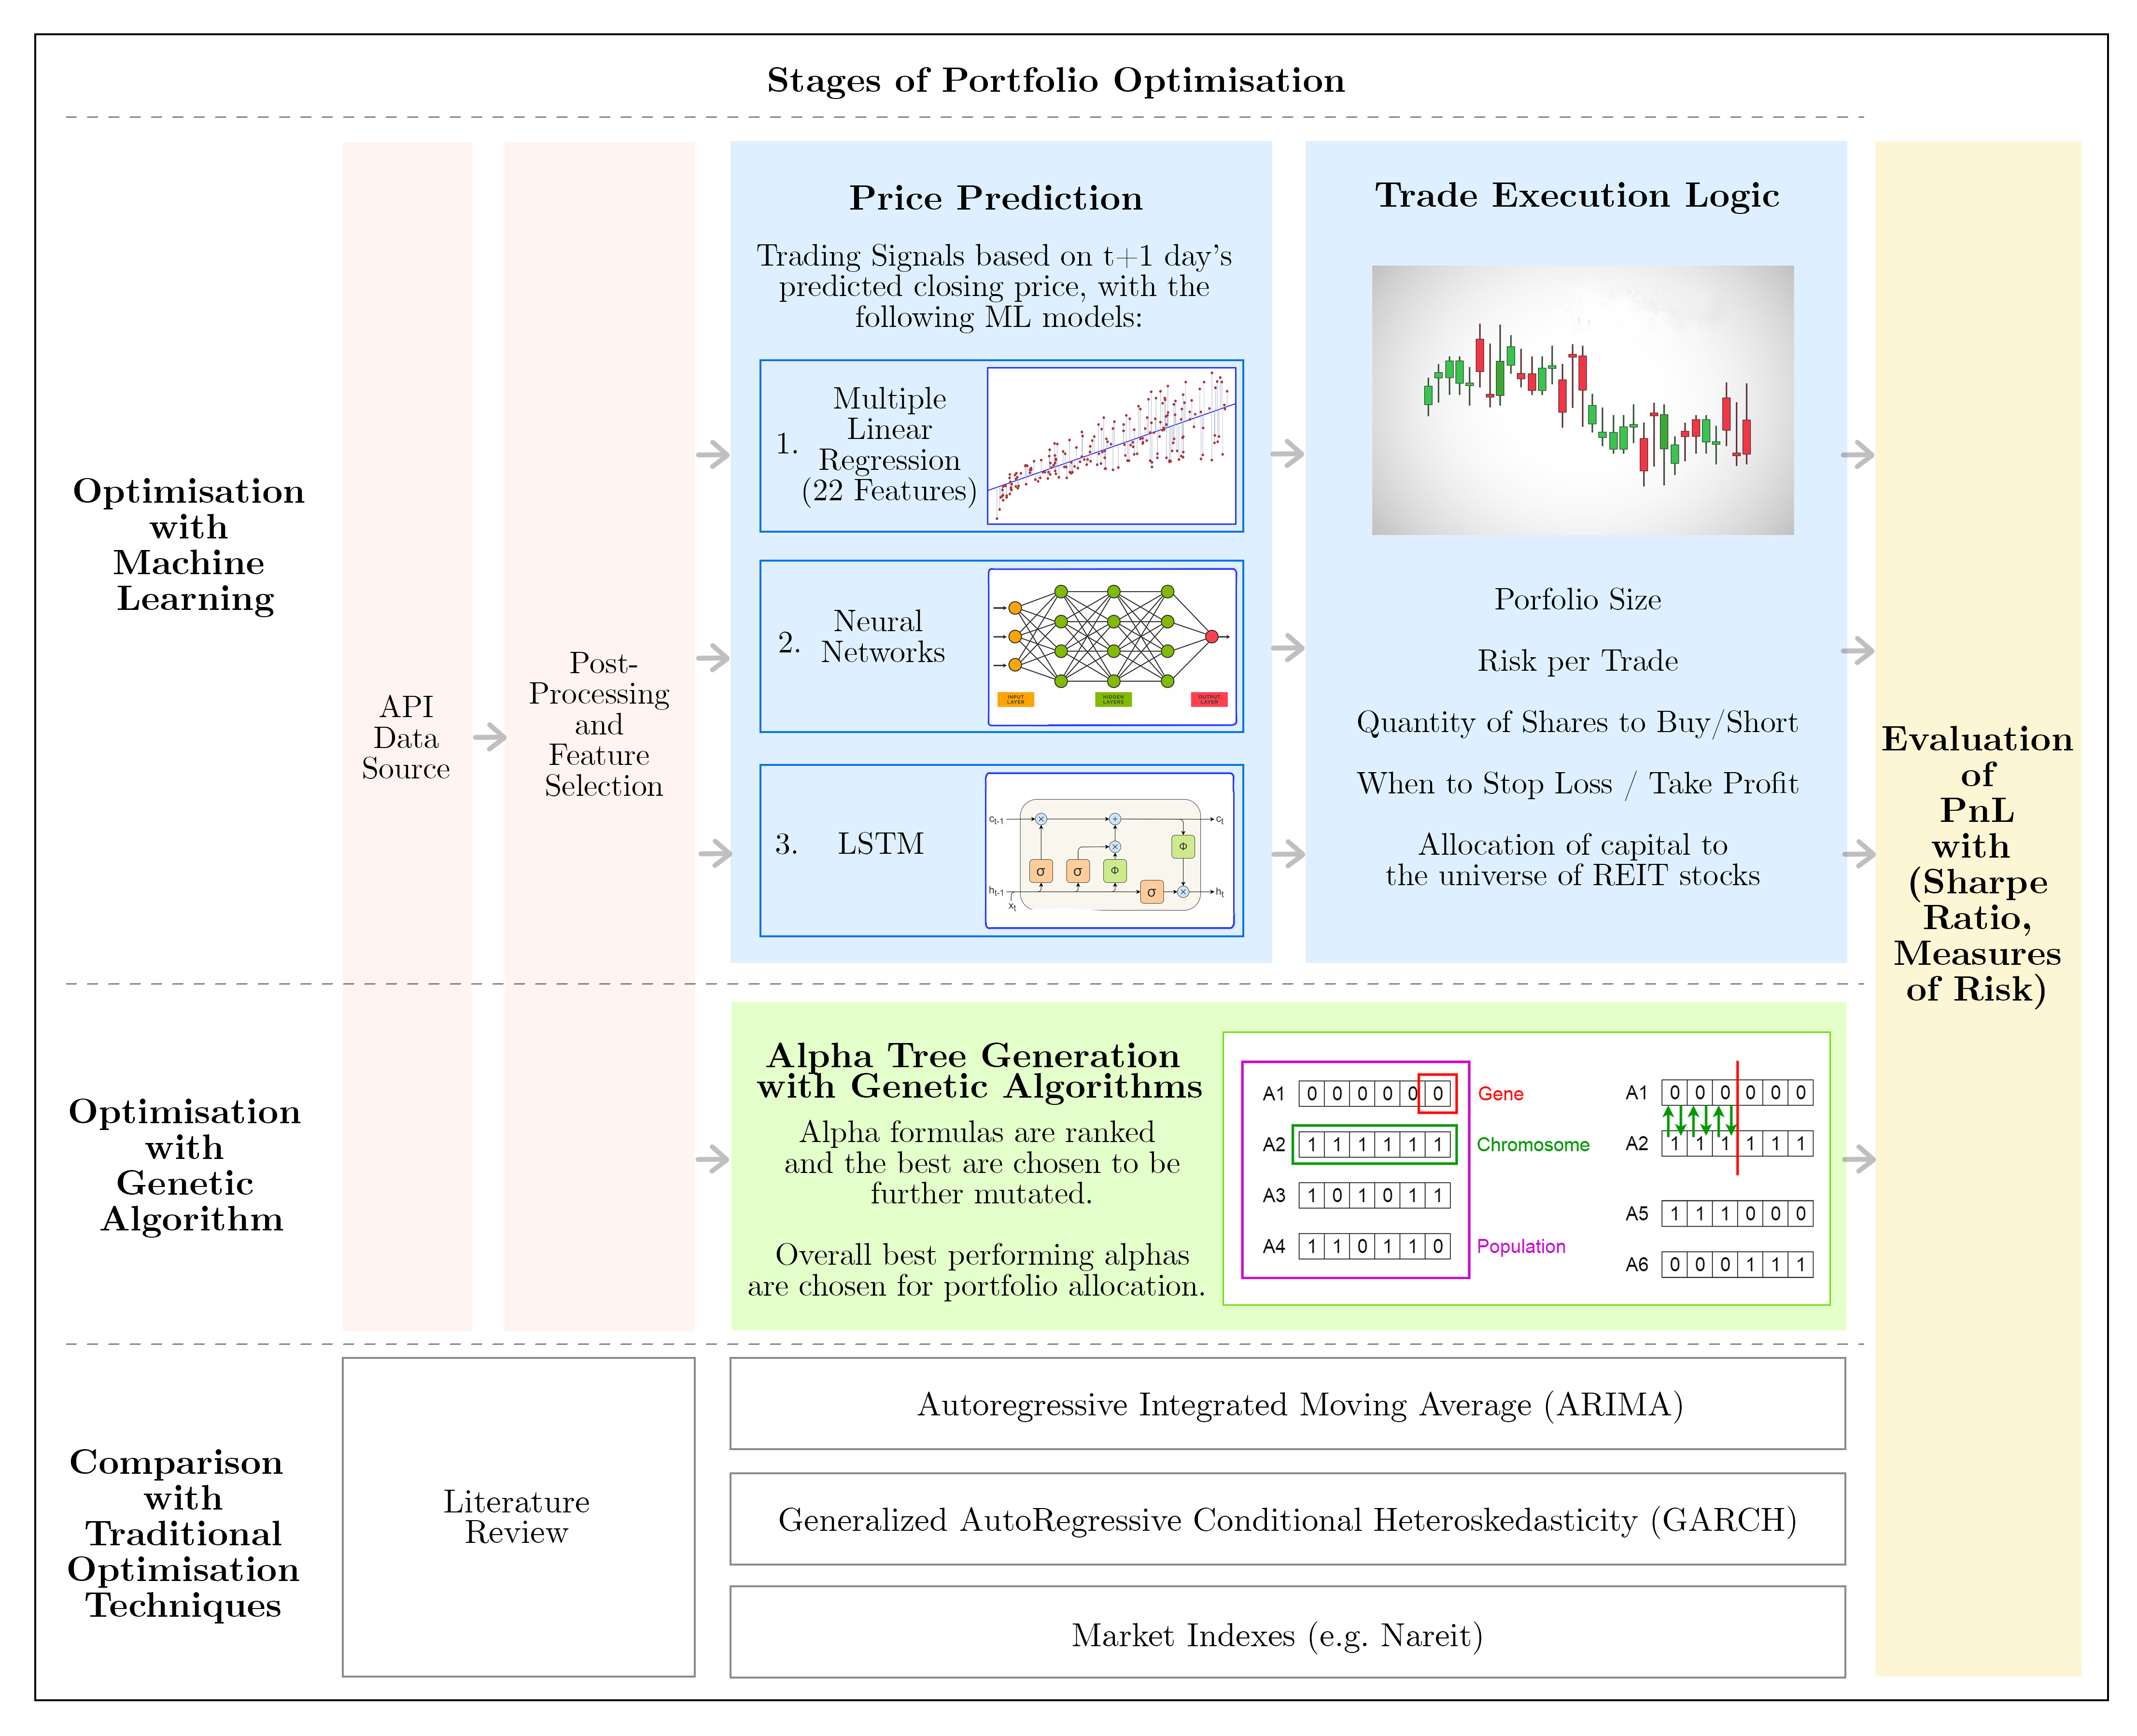
\includegraphics[width=20cm]{Overall_Methodology}}
\caption{Overall Workflow For This Paper}
\label{fig:Overall Workflow For This Paper}
\end{figure}


%\begin{landscape}
%\fillandplacepagenumber
%\end{landscape}

\section{Machine Learning for REITs Portfolio Optimisation}
With reference to Figure \ref{fig:Overall Workflow For This Paper}, the first approach of machine learning for optimisation consists of two parts, A) Price Prediction and B) Trade Execution.


\subsection{MLR / NN / LSTM Predictions with Extended Features}
At the pre-processing stage of all three models, data for each ticker is split into the training and test sets with a 80:20 ratio. The close price for each row is also shifted one day forward so that all 21 features can work on predicting the next day's close.  
\\

By and large, the implementation for all the models are relatively similiar except the lines of code where the model is actually used. The implementation of Multiple Linear Regression is as follows:
\begin{lstlisting}[language=Python, caption=Multiple Linear Regression Pseudocode, basicstyle=\footnotesize\ttfamily]
  for each ticker in dictionary:
      # Training Phase
      X_norm = normalised matrix of 21 features (training set)
      Y_norm = normalised array of T+1 Close Price (training set)
  
      <@\textcolor{red}{model = nn.Linear(21,1) \# Single MLR Layer}@>
      criterion = nn.MSELoss() # MSE Loss Function
      optimizer = optim.SGD(model.parameters(), lr=0.001)

      for epoch in range(10000):
          optimizer.zero_grad()
          Y_pred = model(X_norm)
          loss = criterion(Y_pred, Y_norm)
          loss.backward()
          optimizer.step()

      # Testing Phase
      x_test_norm = normalised matrix of 21 features (test set)
      y_test_norm = normalised array of T+1 Close Price (test set)

      model.eval()
      with torch.no_grad():
        predicted = denormalise(x_test_norm)

      x_test_dates = list of dates from x_test_norm
      df_predicted = pd.DataFrame({
          'Date':x_test_dates,
          'Predicted': pd.DataFrame(predicted)[0].to_list(),
          'Actual': test_set['close'].to_list()
          })
      df_predicted['Actual (t-1)'] = df_predicted['Actual'].shift(1)    
      df_predicted['% Change Predicted'] = (df_predicted['Predicted'] - 
              df_predicted['Actual (t-1)'])/df_predicted['Actual (t-1)']
      df_predicted = df_predicted[['Date','Predicted','Actual',
                                   'Actual (t-1)','% Change Predicted']]
      df_predicted.to_csv('predictions/'+filename+'_pred.csv')
  \end{lstlisting}

Each iteration makes the future stock price predictions for a single ticker over the approximately 5 years of test data based on previous day's inputs. Each ticker will have an output prediction dataframe saved as a csv as follows:
\begin{table}[H]
  \centering
  \caption{Daily Price Prediction for Ticker AHT}
  \begin{tabular}{@{} l *{5}{S[table-format=-1.7]} @{}} 
  \toprule
  {Date} & {Predicted} & {Actual} & {Actual(t-1)} & {\% Change Predicted}\\ % center-set header entries
  \midrule
  26/09/2023    &  110.54  & 111.25 &  111.50 &  -0.0086 \\
  27/09/2023   &  110.33  & 112.13 &  111.25 &  -0.0083 \\
  28/09/2023 &  110.76  & 112.21 &  112.13 &  -0.0122 \\
  \bottomrule
  \end{tabular}
  \label{table:mlr_pred}
\end{table}

\begin{itemize}
  \item {Predicted: Predicted T+1 Day Closing Price}
  \item {Actual: Actual T+1 Day Closing Price}
  \item {Actual(t-1): Today's Closing Price}
  \item {\% Change Predicted: Forecasted \% Change from Today to T+1 Day's Close}
\end{itemize}

For the Neural Network implementation, we swap out the model in the line of code in red in Listing 5.1 and replace it with a the NN model in Listing 5.2.

\begin{lstlisting}[language=Python, caption=Neural Network Model, basicstyle=\footnotesize\ttfamily]
    class NeuralNetwork(nn.Module):
        def __init__(self):
            super(NeuralNetwork, self).__init__()
            self.fc1 = nn.Linear(22, 17)  # First hidden layer
            self.fc2 = nn.Linear(17, 8)   # Second hidden layer
            self.fc3 = nn.Linear(8, 3)    # Third hidden layer
            self.fc4 = nn.Linear(3, 1)    # Output layer
            self.relu = nn.ReLU()         # Activation function

        def forward(self, x):
            x = self.relu(self.fc1(x))
            x = self.relu(self.fc2(x))
            x = self.relu(self.fc3(x))
            x = self.fc4(x)
            return x

    model = NeuralNetwork()
  \end{lstlisting}

This paper has opted for a 3 layer NN model starting from 22 inputs to 17, 8 followed by 3 and uses a Rectified Linear Unit (ReLU) activation function. Likewise it produces the Table \ref{table:mlr_pred} for every ticker.\\

The inputs to the LSTM model are slightly different. A lookback window of 7 days is created by shifting the closing price one day backwards at a time for 7 days to form the additional 7 features as in the Table 5.2.

\begin{table}[H]
  \begin{adjustwidth}{-1.6cm}{-1.6cm}
  \caption{Preprocessed 7 Day Lookback Window for LSTM}
  \begin{tabular}{@{} l *{9}{S[table-format=-1.1]} @{}} 
  \toprule
  {Date} & {Close} & {Close(t-1)} & {Close(t-2)} & {Close(t-3)} & {Close(t-4)} & {Close(t-5)} & {Close(t-6)} & {Close(t-7)}\\ % center-set header entries
  \midrule
  18/12/2023   &  132.68  & 133.75 &  130.47 &  130.96 &  132.40 &  133.46 &  134.18 &  135.19\\
  19/12/2023 &  133.75 & 130.47 &  130.96 &  132.40 &  133.46 &  134.18 &  135.19 & 133.30\\
  \bottomrule
  \end{tabular}
  \end{adjustwidth}  
  \label{table:lstm_close_shift2}
\end{table}

These prior days closing prices are appended to the 22 features input into the LSTM model. The line of code in red in Listing 5.1 is also replaced with an LSTM model in Listing 5.3. 

\begin{lstlisting}[language=Python, caption=LSTM Model, basicstyle=\footnotesize\ttfamily]
  class LSTM(nn.Module):
    def __init__(self, input_size, hidden_size, num_stacked_layers):
        super().__init__()
        self.hidden_size = hidden_size
        self.num_stacked_layers = num_stacked_layers

        self.lstm = nn.LSTM(input_size, hidden_size, 
                            num_stacked_layers,
                            batch_first=True)

        self.fc = nn.Linear(hidden_size, 1)

    def forward(self, x):
        batch_size = x.size(0)
        h0 = torch.zeros(self.num_stacked_layers, batch_size, 
                         self.hidden_size).to(device)
        c0 = torch.zeros(self.num_stacked_layers, batch_size, 
                         self.hidden_size).to(device)

        out, _ = self.lstm(x, (h0, c0))
        out = self.fc(out[:, -1, :])
        return out

  model = LSTM(1, 4, 1)
\end{lstlisting}

All 3 models produce a daily price prediction file for each of the 150 tickers in the format shown in Table \ref{table:mlr_pred}. With the daily future price predictions, 

\subsection{Trade Execution Logic}
The second part of the machine learning approach requires implementing the logic to decide how to trade on these predictions. This extends past research by implementing the trading logic that decides how to act on predicted prices in order to optimise portfolios. \\

All the predicted prices for all the dataframes are appended into a single large data frame, the parameters as follows are set and the green columns in Figure \ref{fig:trade_execution_amount} are computed.

\begin{lstlisting}[language=Python, caption=Parameters for Trade Execution, basicstyle=\footnotesize\ttfamily]
  action_threshold = 0.03
  stop_loss_percentage= 0.05
  take_profit_percentage = 0.15
  trade_factor_denominator = 0.20
  shorting_enabled = True
\end{lstlisting}

\begin{figure}[H]
  \centerline{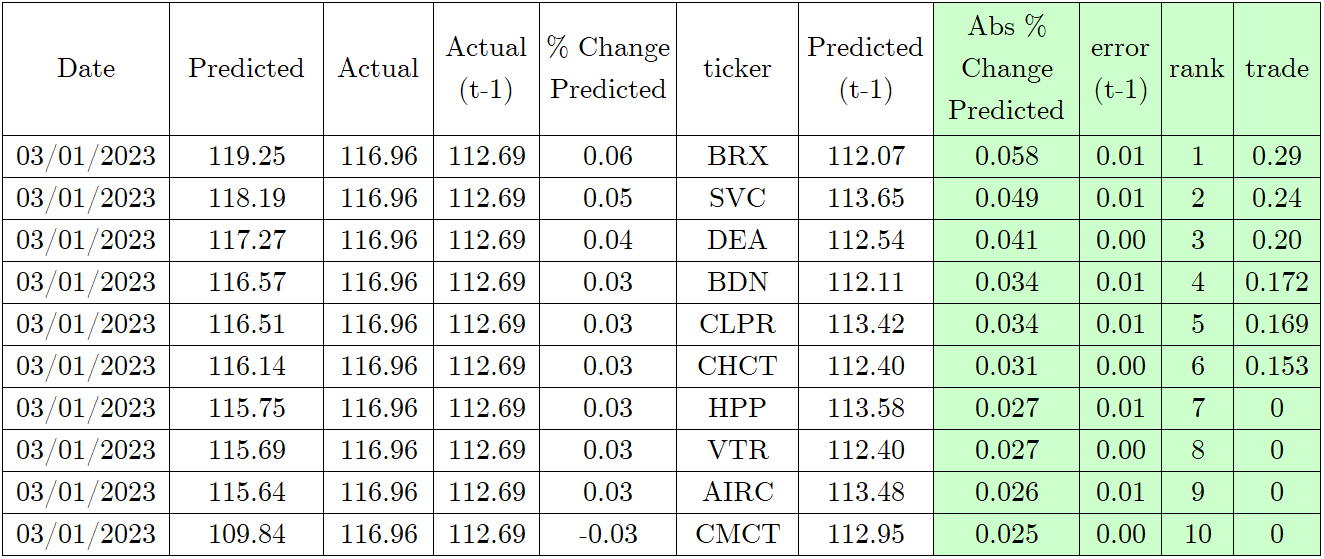
\includegraphics[width=17cm]{determining_trade_amount}}
  \caption{Processing Predicted Prices to Determine Trade Amount}
  \label{fig:trade_execution_amount}
\end{figure}

\begin{itemize}
  \item {Predicted (t-1): Yesterday's Predicted (T-1 of Predicted)}
  \item {Abs \% Change Predicted: $abs(\% Change Predicted)$}
  \item {error (t-1): Difference Between Yesterday's Predicted and Actual}
  \item {rank: Rank of all 150 Ticker's Abs \% Change Predicted}
  \item {trade: If Abs \% Change Predicted exceeds the action\_threshold parameter, trade an amount equal to \% Change Predicted / trade\_factor\_denominator in millions. If shorting is disabled, does not take action on negative \% Change Predicted.}
\end{itemize}

Next, a transaction class is defined to store the historical price of the original transaction until the position is closed.

\begin{lstlisting}[language=Python, caption=Transaction Class Pseudocode, basicstyle=\footnotesize\ttfamily]
Class Transaction (Date, Actual(T-1), trade, max_allocation_per_trade): 

    Store as members:
      - Total Original Trade Amount
      - Initial buy/sell price
      - Initial buy/sell quantity
      - Initial buy/sell date
      - Ending sell/buy price
      - Ending sell/buy date
      - PnL from this transaction
      - Whether the position is closed (Boolean)

    Method Action (today_actual_price, today_date) 

        If position is open,
            compute % change from initial buy/sell to today's price.
        
            <@\textcolor{blue}{If the position was originally long*, }@> 
                <@\textcolor{blue}{If the percentage loss > stop\_loss\_percentage, }@> 
                    <@\textcolor{blue}{execute stop loss and sell position at today's price. }@>  

                <@\textcolor{blue}{If the percentage gain > take\_profit\_percentage, }@>
                    <@\textcolor{blue}{take profit and close the position at today's price. }@>      

                    (In both instances record the date, price and 
                    profit from the closing transaction) 

            *If the position was originally short, 
                do the inverse of the section in blue.
 
\end{lstlisting}
For every non-zero Trade amount in Figure \ref{fig:transaction_objects}, the transaction class is called with the required inputs and a transaction object is created in yellow.
\begin{figure}[H]
  \centerline{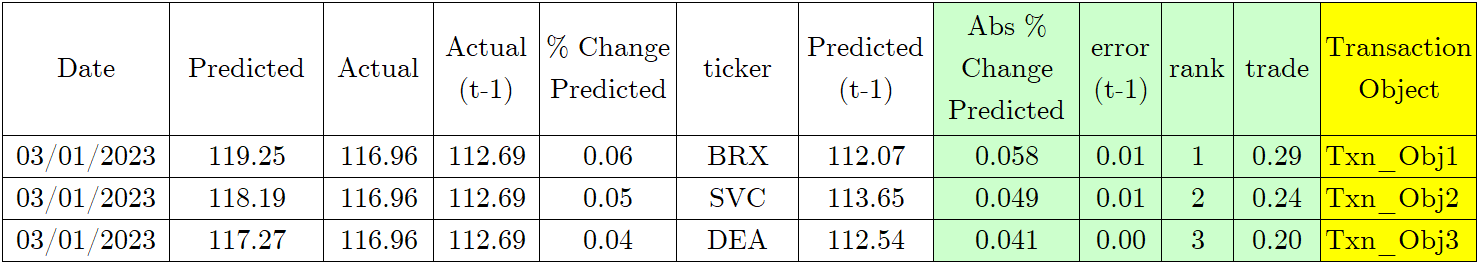
\includegraphics[width=17cm]{transaction_objects}}
  \caption{Calling the Transaction Class to Create Transaction Objects}
  \label{fig:transaction_objects}
\end{figure}
The closing transaction details are then added to each transaction object by iterating through the ticker's price movement over time and calling the Action method of the transaction class, which will close the position when the conditions in Listings 5.5 are met. 
\subsection{Performance Evaluation}
In the evaluation phase the various dataframes will be consolidated to calculate the following time series from the start to the end of the test data:
\begin{enumerate}
  \item {The total daily value of each ticker over the entire period}
  \item {The daily cash balance which started at 10 million}
  \item {The daily total portfolio value = Sum of all the daily ticker values in point 1. and daily cash balances in point 2.}
\end{enumerate}

\underline{Expected Return}:
Following which the total expected return from the investment is calculated as follows:

\begin{equation*}
  Amount\,Invested\,=\,Minimum\,cash\,balance\,across\,investment\,horizon 
\end{equation*}  

\begin{equation*}
  Expected\,Total\,Return\,=\,\frac{Average\,Daily\,Portfolio\,Value\,-\,Amount\,Invested}{Amount\,Invested}
\end{equation*}

\underline{Annualised Rate of Return}:
\begin{equation*}
  Annualised\,Rate\,of\,Return\,(R_p)\,=\,(Expected\,Total\,Return)\,^{\frac{1}{investment\,horizon\,in\,years}}
\end{equation*}  


\underline{Standard Deviation}:
\begin{equation*}
  \rho_p = deviation\,of\,portfolio\,array\,divided\,by\,cash\,for\,each\,date
\end{equation*}  

\underline{Sharpe Ratio}:
\begin{equation*}
  Sharpe\,Ratio\,=\,\frac{R_p\,-\,Average\,Risk\,Free\,Rate}{\rho_p}
\end{equation*}  



\section{Genetic Algorithm (GA) Search for Outperforming Alphas}
The second approach is inspired by Charles' Darwin theory of evolution in Figure \ref{fig:giraffes}. In the context of Alphas and portfolio allocation, this paper hypothesizes that a combination of trading formulas that outperform may result in even better performing Alphas.  Such a trading algorithm would  simulate the process of natural selection in the real world, by choosing the best performing members of the population for reproduction in order to produce the next generation.

\begin{figure}[H]
  \centerline{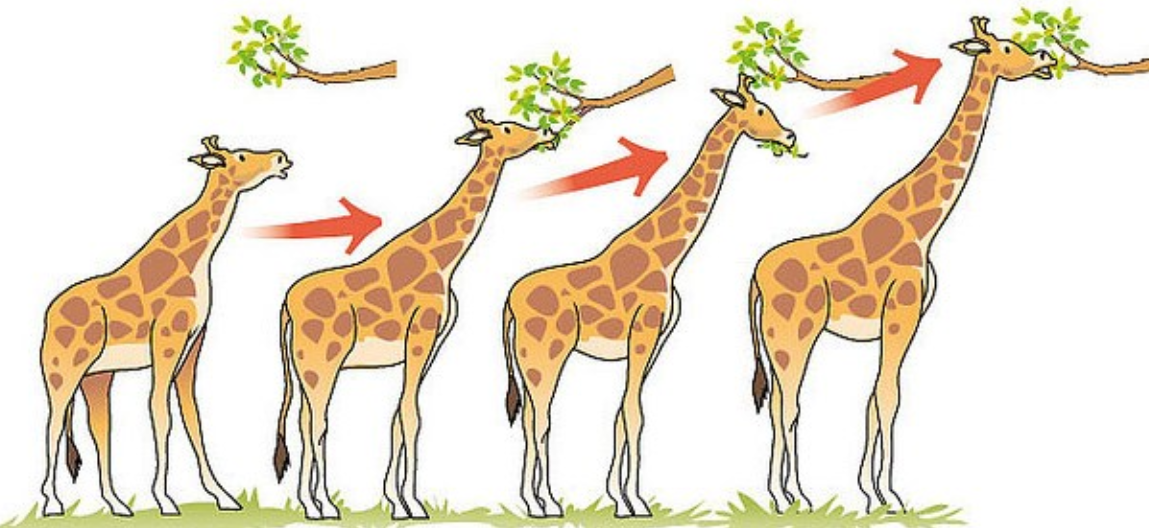
\includegraphics[width=14cm]{giraffes}}
  \caption{Giraffes with longer necks are able to reach higher for food making them more likely to survive and reproduce, resulting in children with longer and longer necks because this trait is successful in this environment. (Image Source: Wikipedia) }
  \label{fig:giraffes}
\end{figure}

\subsection{Alpha Tree}
This paper represents and implements Alphas with a Tree like in Figure \ref{fig:alpha_tree_first}. 
\begin{figure}[H]
  \centerline{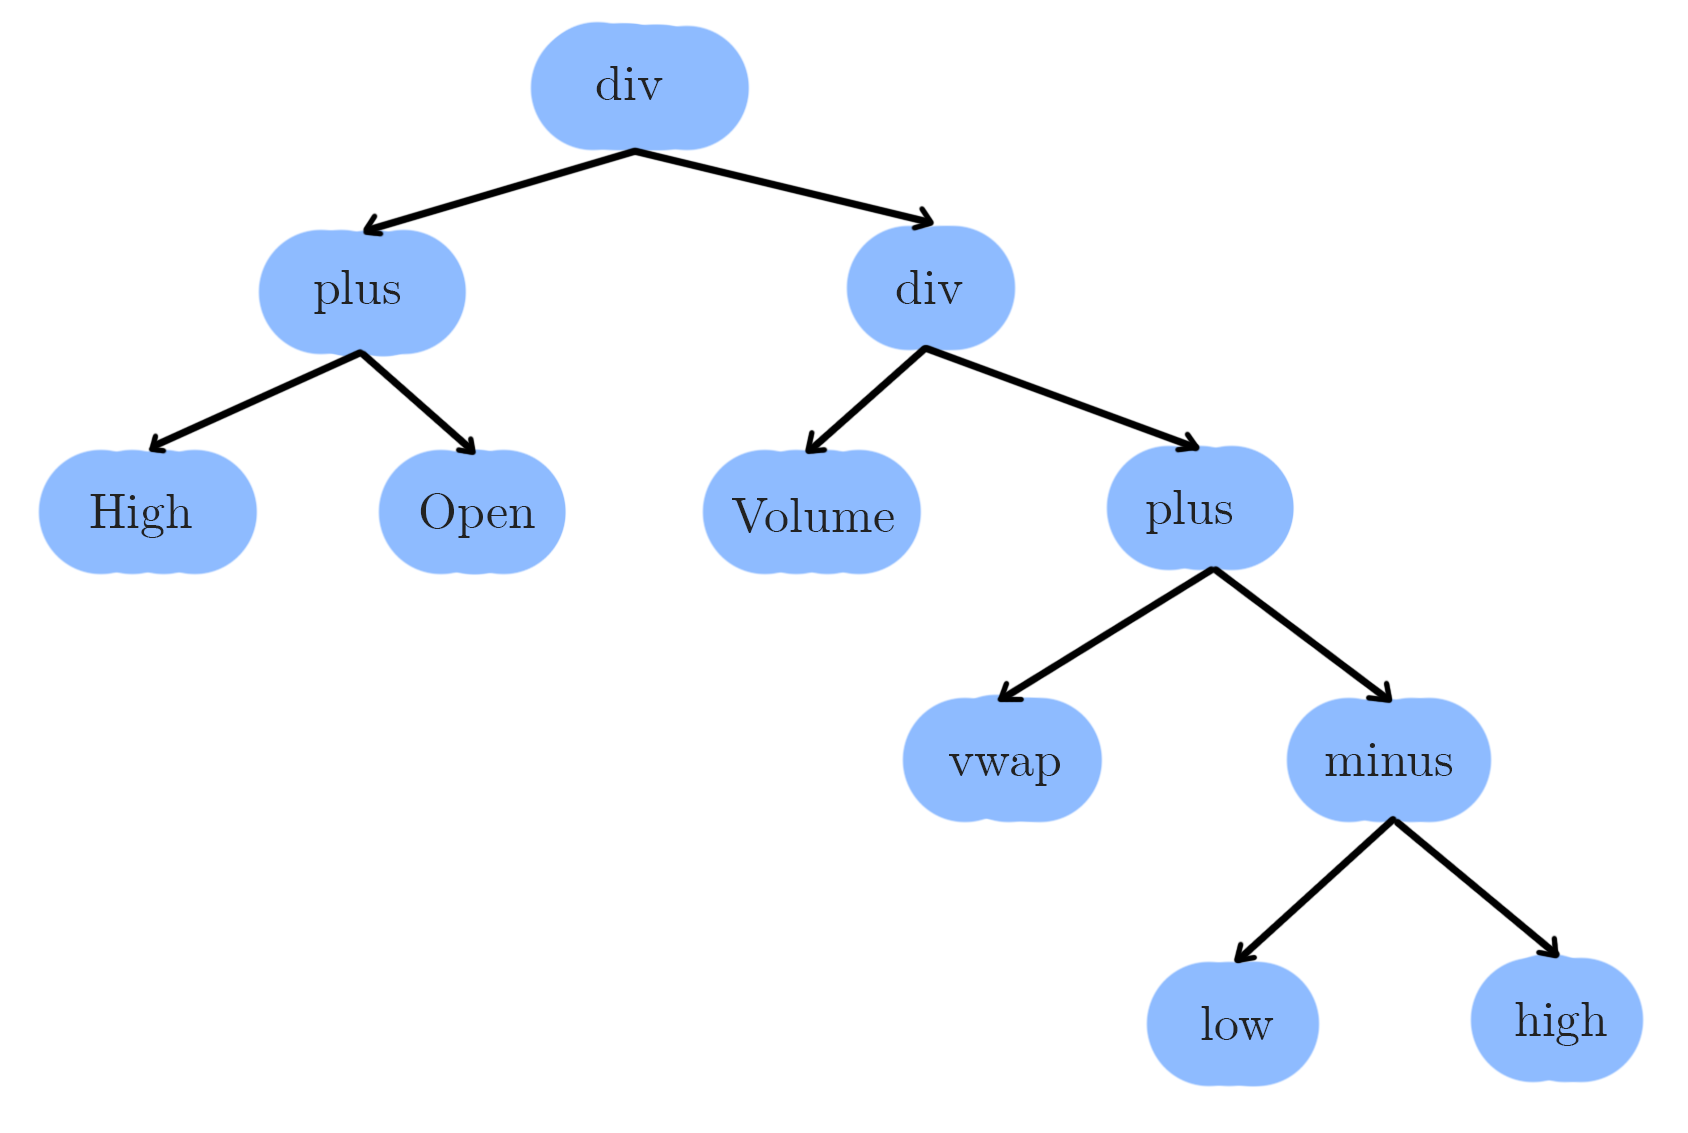
\includegraphics[width=12cm]{alpha tree first}}
  \caption{(high + open)/(volume/(vwap+low-high))}
  \label{fig:alpha_tree_first}
\end{figure}
In using the GA to search for outperforming Alpha Trees, two good performing parents are selected and combined to form a new child. The parents are split at a randomised part of the tree before being recombined with each other. This is illustrated in Figure \ref{fig:alpha_tree_second}.
\begin{figure}[H]
  \centerline{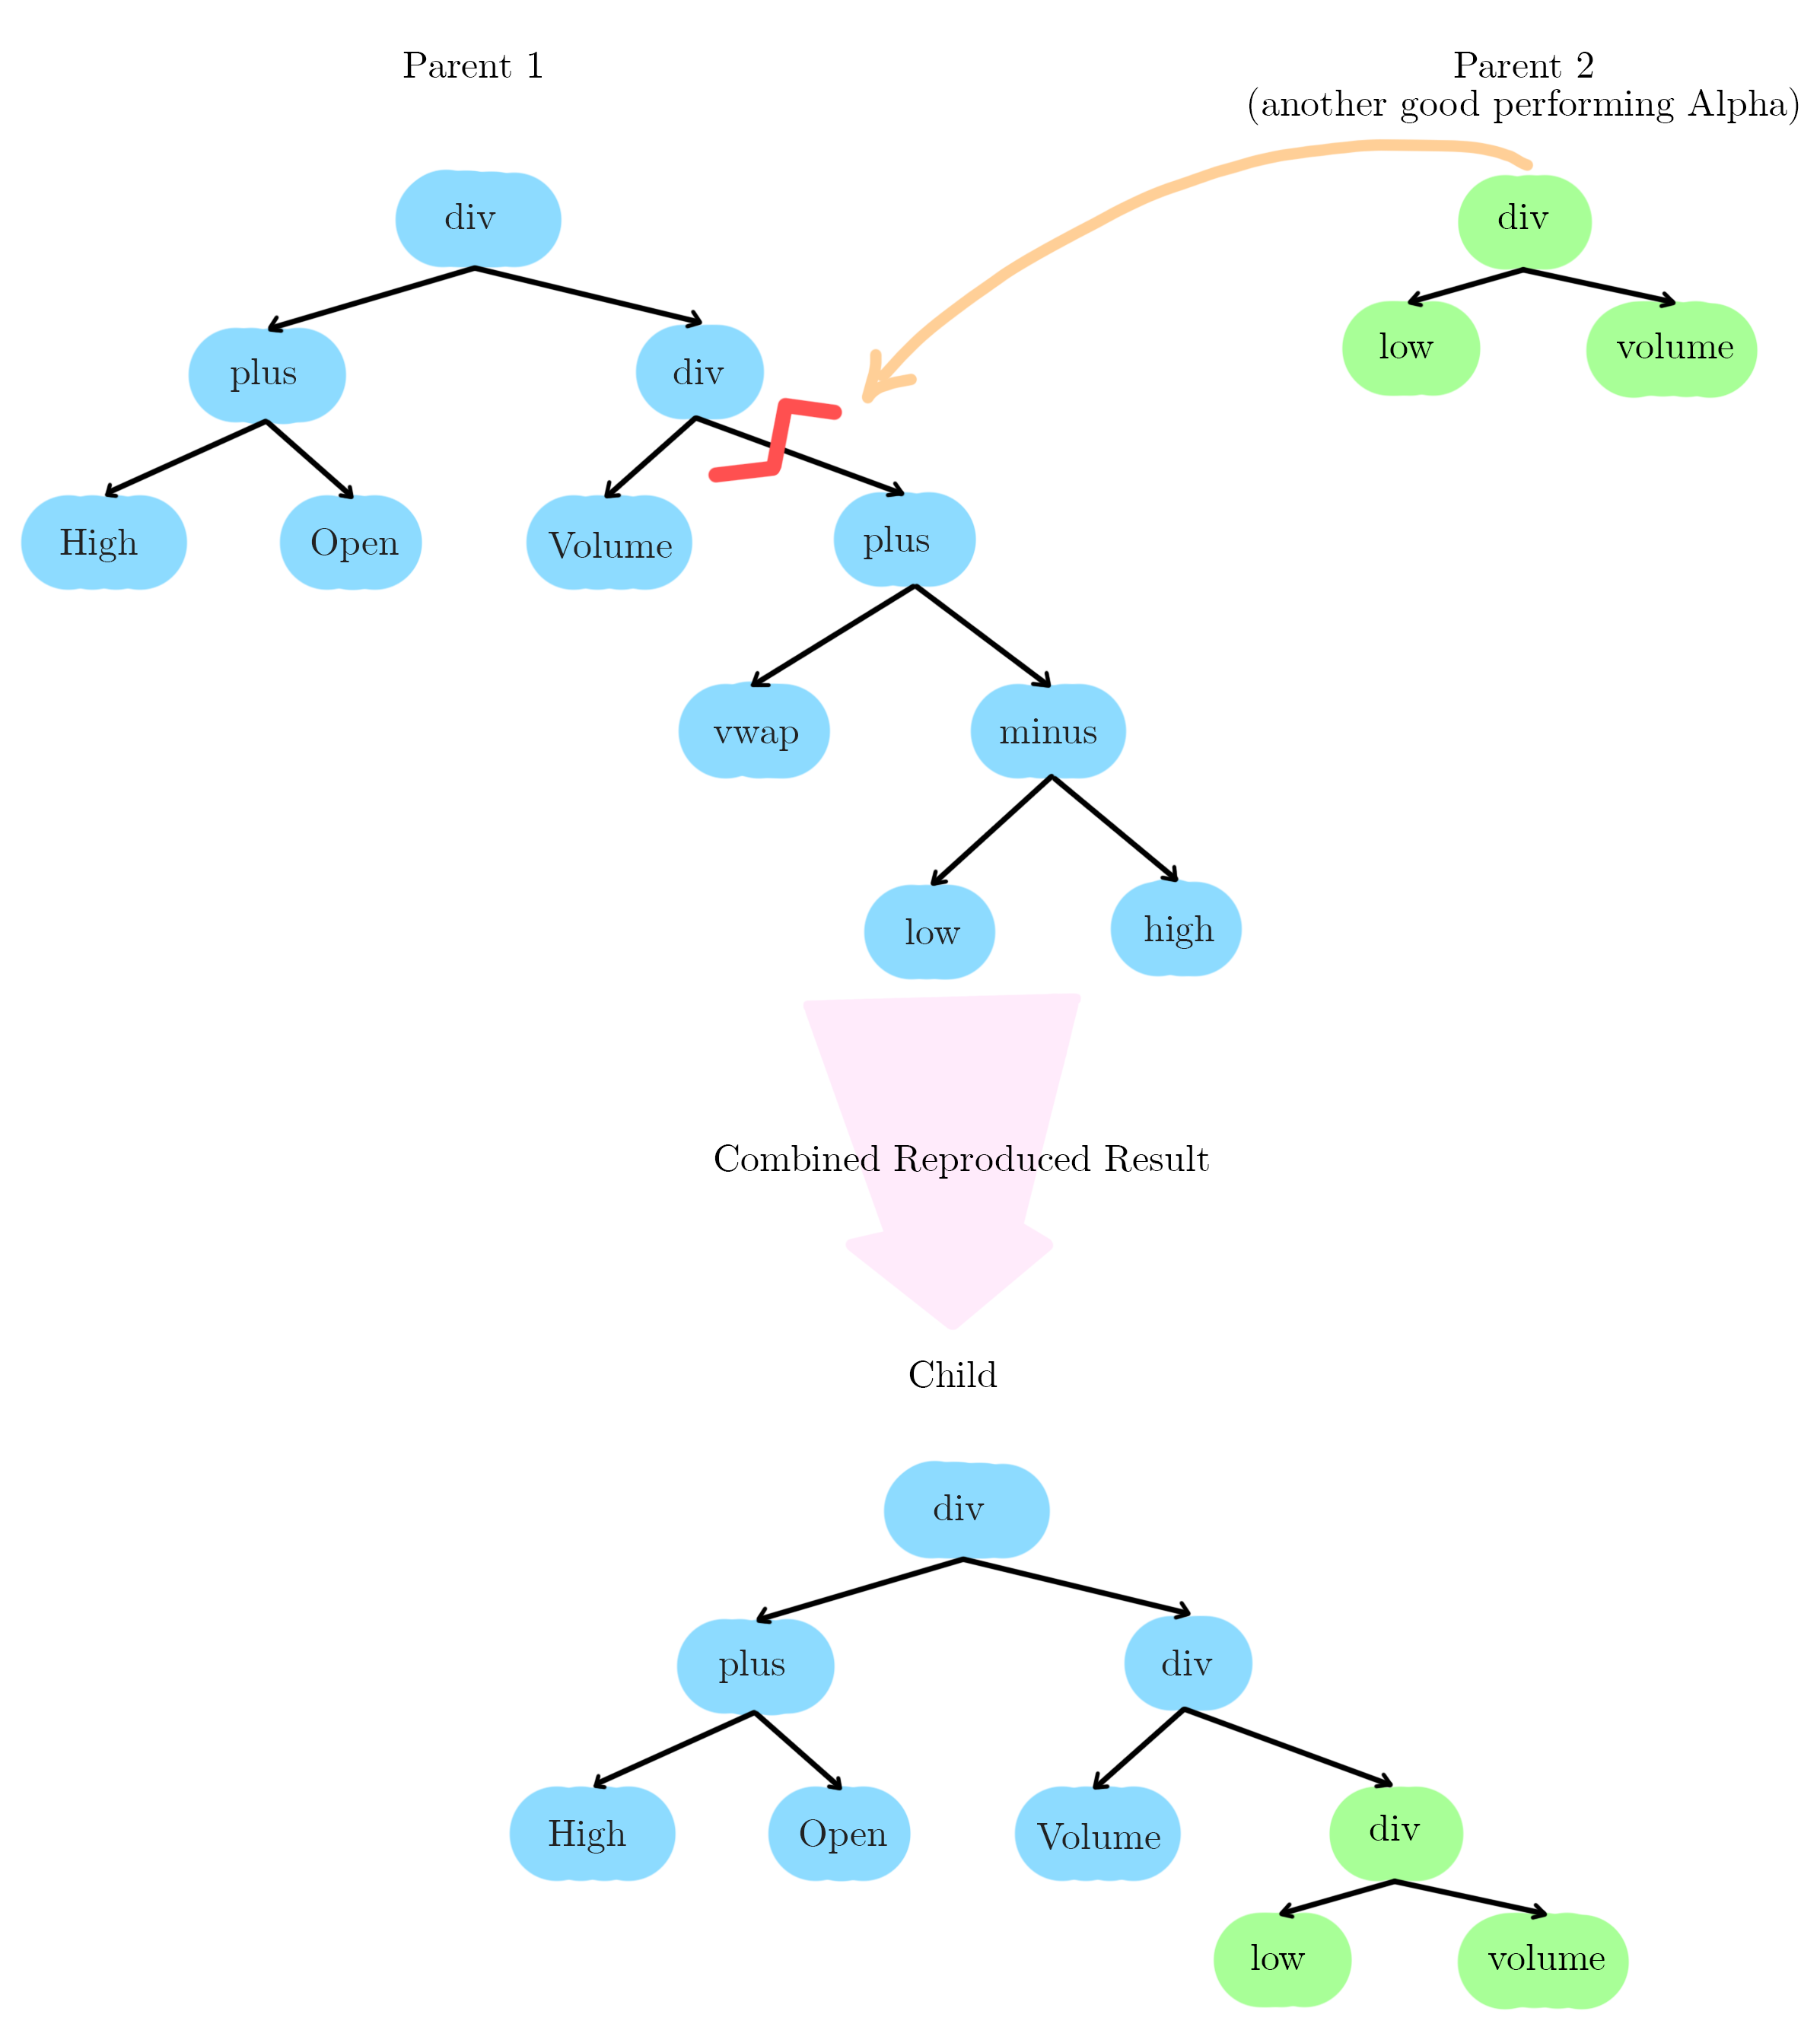
\includegraphics[width=15cm]{alpha tree second}}
  \caption{Reproduction Between Two Alphas}
  \label{fig:alpha_tree_second}
\end{figure}

\subsection{Application of Genetic Algorithms to Alpha Trees}
In order to implement the ideas in Section 5.2.1, a series of functions in the following subsections are created.
\subsubsection{Generate Starting Population}
The function in Listing 5.6 generates the first population of Alphas from which the GA will work on.

\begin{lstlisting}[language=Python, caption=Generate Starting Alphas Pseudocode, basicstyle=\footnotesize\ttfamily]
  datafields = ['Open','Close','High','Low','Volume'] 
  operators = ["+", "-", "*", "/"]
  number = 10 # Number of Alphas in the starting population
  
  def generateAlphas(number,datafields,operator):
    # Randomly combines operators and fields to form Alphas
    return List of randomly generated Alphas 
  \end{lstlisting}


\subsubsection{Objective Function}
The objective function evaluates the average profit of an Alpha over a one year period with a 1\% transaction cost factored in to determine its performance. 

\begin{lstlisting}[language=Python, caption=Objective Function Pseudocode, basicstyle=\footnotesize\ttfamily]
  def objectve(tickers_price_data,Alpha):
      Calculate one year, six month, three month and 
      one month returns from the latest date. 
      return average of these returns
  \end{lstlisting}

\subsubsection{Selection}
The selection function defines how parent Alphas are selected from the population. 
\begin{lstlisting}[language=Python, caption=Selection Function Pseudocode, basicstyle=\footnotesize\ttfamily]
  pop = array of alphas
  scores = scores for each alpha member from objective function
  k = number of alphas to select
  def selection(pop,scores,k=3):
      Select k number of alphas from the population 
      to compare scores against each other 
      return the alpha with the greatest score
\end{lstlisting}

\subsubsection{Crossover}
Next, the Crossover function, which is the core of the GA and implements the reproduction between parents to produce an offspring.
\begin{lstlisting}[language=Python, caption=Crossover Function Pseudocode, basicstyle=\footnotesize\ttfamily]
  r_cross = probability of crossover occuring
  def crossover(parent1,parent2,r_cross):
    if probability exceeds r_cross:
      # Crossover occurs
      for each parent p1 and p2:
        slice parents into left and right at a valid intersection
        ensure equal number of left and right brackets, 
        append brackets if neccesary
      child1 = parent1 left + parent2 right
      child2 = parent2 left + parent1 right
      return [child1,child2]
    else:
      # No crossover
      return [parent1,parent2]
\end{lstlisting}

\subsubsection{Mutation}
Followed by a crossover function which determines at rate at which certain datafields are mutated (i.e. randomly changed to another valid datafield).
\begin{lstlisting}[language=Python, caption=Mutation Function Pseudocode, basicstyle=\footnotesize\ttfamily]
  r_mut = probability of mutation occuring
  def mutation(alpha,fields,r_mut):
    for each feature in datafields:
      if probability exceeds r_mut:
        Search Alpha for feature and replace it randomly
    return mutated Alpha
\end{lstlisting}

\subsubsection{Genetic Algorithm}
The overall GA function which calls the various parts above is as follows:
\begin{lstlisting}[language=Python, caption=Genetic Algorithm Pseudocode, basicstyle=\footnotesize\ttfamily]
define genetic_algorithm(objective_function, datafields, 
                          n_iter, n_pop, r_cross, r_mut):

# Randomly generate the initial population
pop = generateAlphas(number,datafields,operator)

# Keep track of best Alpha and objective score
best, best_eval

for each iteration in n_iter:
  scores = [objective(alpha) for alpha in pop]

  # Check for new best solution
  for member in pop:
    if score of member > best_eval:
      best = member
      best_eval = member score

  # Select parents
  select n_pop number of parents using selection function on pop

  # Create next generation
  new_pop = run crossover and mutation functions on selected parents

  # Replace old pop with new pop and move to next iteration
  pop = new_pop

# After all iterations are complete, return the best alpha
return best,best_eval
\end{lstlisting}

\subsection{Portfolio Allocation Using Alpha}
The best Alpha returned from the GA is applied in the manner explained in Figure \ref{fig:alpha table} to create the column in yellow as illustrated in Figure \ref{fig:pnl_table}. By taking the cumulative sum of the yellow column we create the column in green.
\begin{figure}[H]
  \centerline{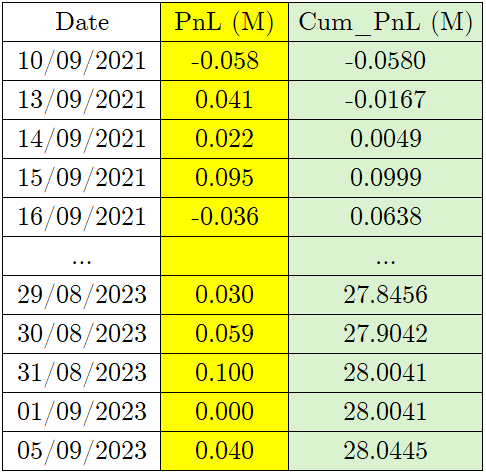
\includegraphics[width=7cm]{pnl}}
  \caption{Daily and Cumulative PnL}
  \label{fig:pnl_table}
\end{figure}

The latest number in the green column represents the total profit on investment. 
\subsection{Performance Evaluation}


The method of measuring performance is the same used in the Machine Learning approach, save for slight changes to the equation for Expected Total Return

\begin{equation*}
  Amount\,Invested\,=\,20\,Million
\end{equation*}  
\underline{Expected Return}:
\begin{equation*}
  Expected\,Total\,Return\,=\,\frac{Total\,Profit\,on\,Investment\,+\,Amount\,Invested}{Amount\,Invested}
\end{equation*}



\titleformat{\chapter}[block]
  {\normalfont\huge\bfseries}{\thechapter.}{1em}{\Huge\centering}
\titlespacing*{\chapter}{0pt}{230pt}{0pt}
\setcounter{chapter}{2}
\renewcommand{\thechapter}{\Roman{chapter}}
\chapter{Experiments}

\titleformat{\chapter}[display]{\Large}{\centering
  \MakeUppercase{\chaptername}\quad{\Huge\thechapter}}{10pt}{\titlerule[.5pt]\vspace{10pt}\centering
  \MakeUppercase}[\vspace{10pt}{\titlerule[.5pt]}]% <-- spacing of title bar
\titlespacing{\chapter}{0pt}{-23pt}{1cm}% <-- spacing of title bar
\renewcommand{\thechapter}{\arabic{chapter}}
\setcounter{chapter}{5}
\pagenumbering{arabic}












\begin{landscape}
\chapter{Post-processed Financial Dataset}
Figure \ref{fig:post_processed_data} presents a sample of the post-processed data for a single Ticker of its 23 fundamental and technical features. This extends the analysis beyond the usual price-volume data used in ML. Data for 150 tickers and up to 20 years are used to train the models.
\begin{figure}[H]
  \centerline{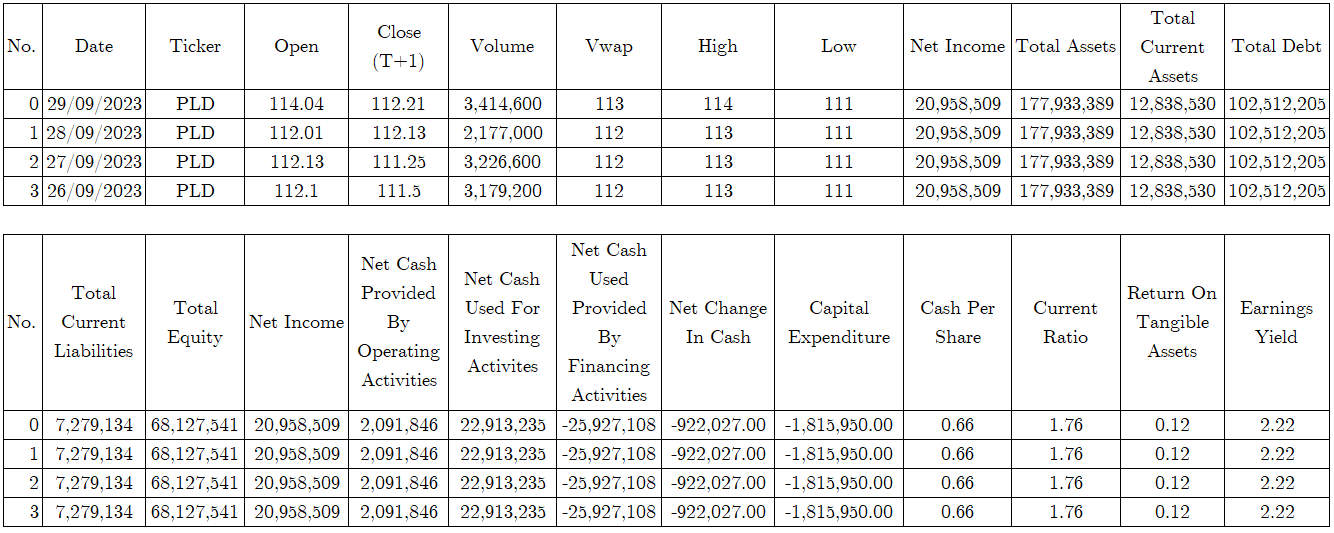
\includegraphics[width=23cm]{post-processed data}}
  \caption{Input Features for ML Models}
  \label{fig:post_processed_data}
\end{figure}

\end{landscape}

\chapter{Machine Learning Results}
This section presents the results of porfolio allocation using MLR, NN and LSTM models. 
\section{Evaluating Stock Price Predictions}
In terms of the first part of the ML approach of stock price prediction, it appears all 3 models have predicted prices that closely mirror the actual prices in Figure \ref{fig:PLD_price_pred}.
\begin{figure}[H]
  \centerline{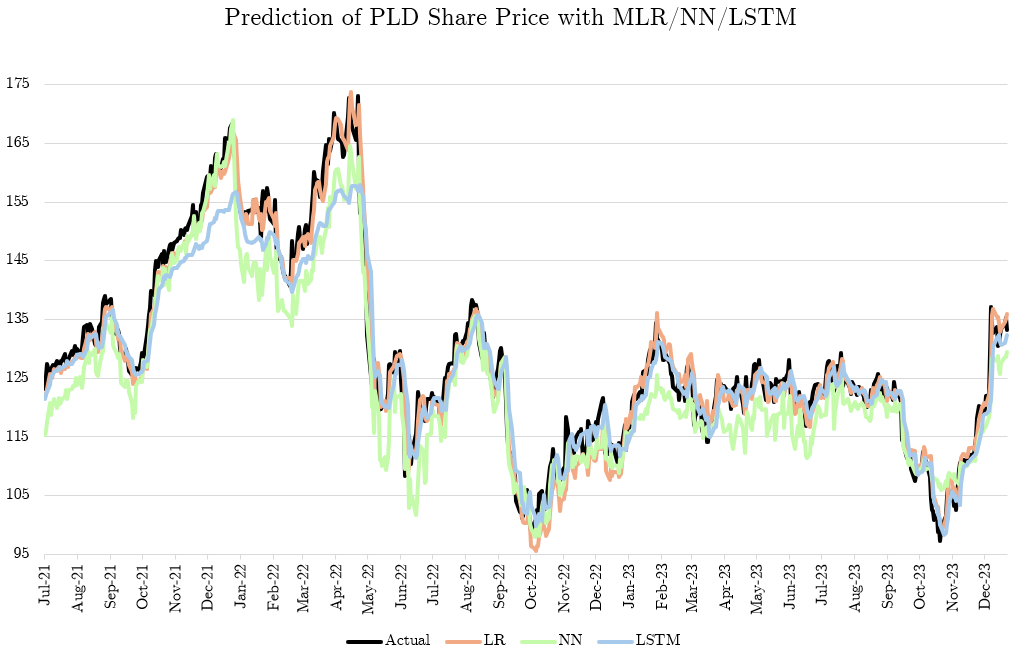
\includegraphics[width=17cm]{ML Predictions PLD Price}}
  \caption{PLD Share Price Predicted vs Actual}
  \label{fig:PLD_price_pred}
\end{figure}
However, comparing their Mean Square Errors (MSE) reveals that LSTM provides the most accurate price prediction, followed by NN and then LR, with a MSE of 212, 252 and 323 respectively in Figure \ref{fig:MSE_ML}. 
\begin{figure}[H]
  \centerline{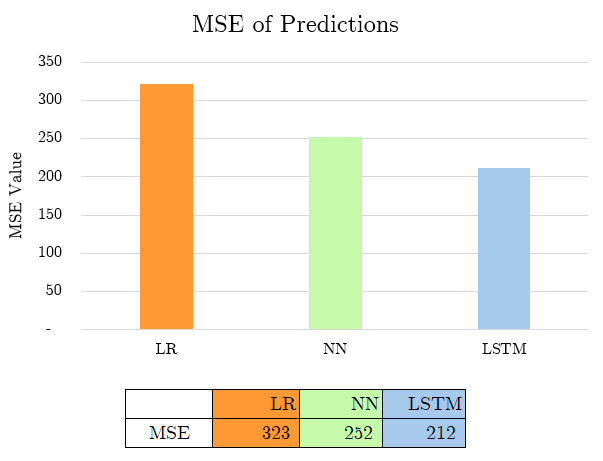
\includegraphics[width=13cm]{MSE of ML models}}
  \caption{Mean Squared Error of Prediction Models}
  \label{fig:MSE_ML}
\end{figure}
It appears that even while including fundamental data features, LSTM's memory of historical price information does aid its ability to identify trends and make more accurate predictions (Obthong et. al.,2020). And NN's multiple layers help to further reduce the error in predictions.

\section{Trade Execution Results with Different Parameters}
In the second phase of the ML approach, the buy/sell decisions are made based on the predicted prices. Using MLR as an example, where shorting is not allowed, the total value of each ticker after trade execution over the test period from 2019 to 2024 is shown in Figure \ref{fig:portfolio_movement}.

\begin{figure}[H]
  \centerline{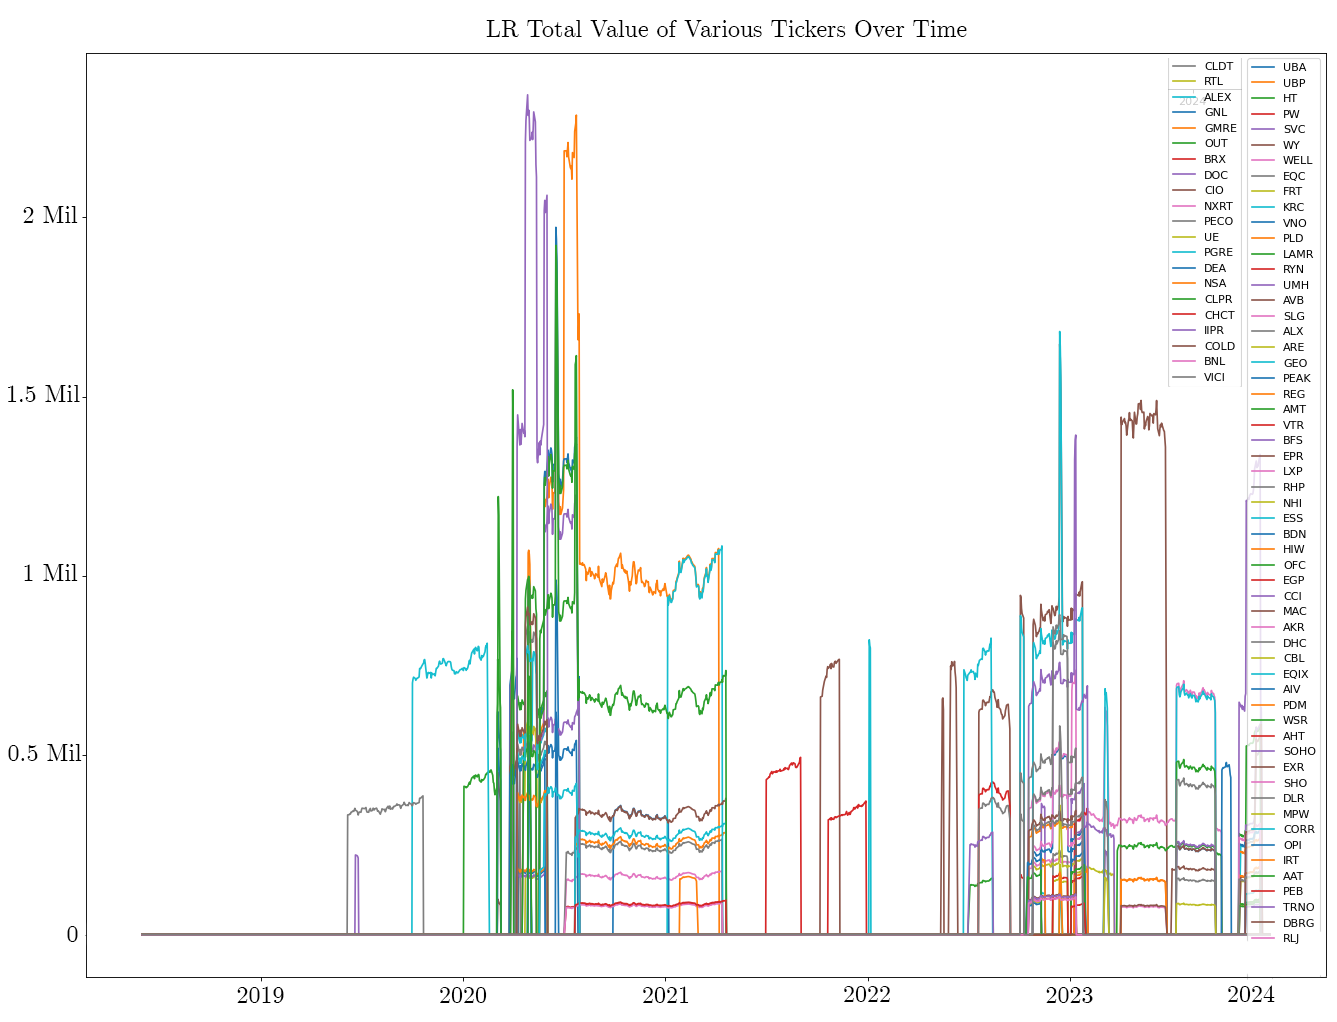
\includegraphics[width=16cm]{ML_portfolio_value_movement}}
  \caption{Value of Each Ticker As Portfolio Allocation Occurs Over The Period}
  \label{fig:portfolio_movement}
\end{figure}

Each line in Figure \ref{fig:portfolio_movement} represents the total value of one out of the 150 investible tickers throughout the portfolio allocation period. Correspondingly, the cash balances after various stock tickers are bought or sold is given in Figure \ref{fig:Cash Balance of Portfolio}. The sum of the total daily value of stocks and the cash balance for the day will result in Figure \ref{fig:Total portfolio Value}, which is the total portfolio value throughout the investment horizon.\\

The Figures show an inverse relationship between cash balances and value of shares held because cash is traded for shares. The total portfolio value was maintained consistently above the starting investment of 10 Million, although it spiked in early 2020 and fell sharply thereafter. It is worthy to note that the COVID-19 pandemic started to seriously impact the financial markets in mid-2020 which coincided with the total fall in portfolio value. \\

The same trade execution logic is implemented for NN and LSTM as well, generating the total portfolio value graph in Figure \ref{fig:Total portfolio Value}, upon which porfolio performance is evaluated.

\begin{figure}[H]
  \centerline{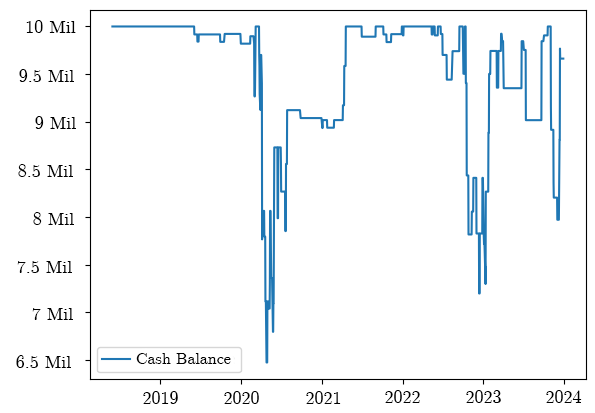
\includegraphics[width=13cm]{LR Cash Balance}}
  \caption{Cash Balance of Portfolio Over The Period}
  \label{fig:Cash Balance of Portfolio}
\end{figure}

\begin{figure}[H]
  \centerline{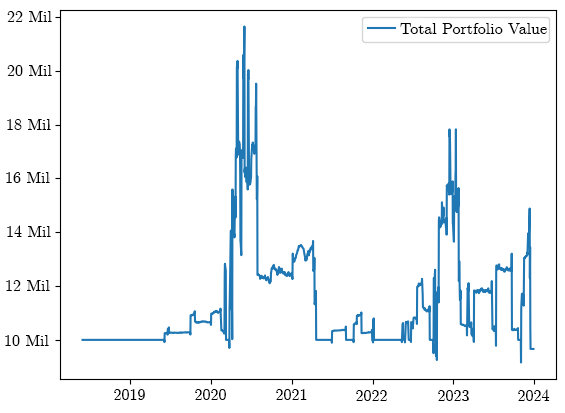
\includegraphics[width=13cm]{Total Portfolio Value LR}}
  \caption{Total Portfolio Value (Stocks + Cash) Over Time}
  \label{fig:Total portfolio Value}
\end{figure}



\section{Overall Evaluation of Performances}

\begin{figure}[H]
  \centerline{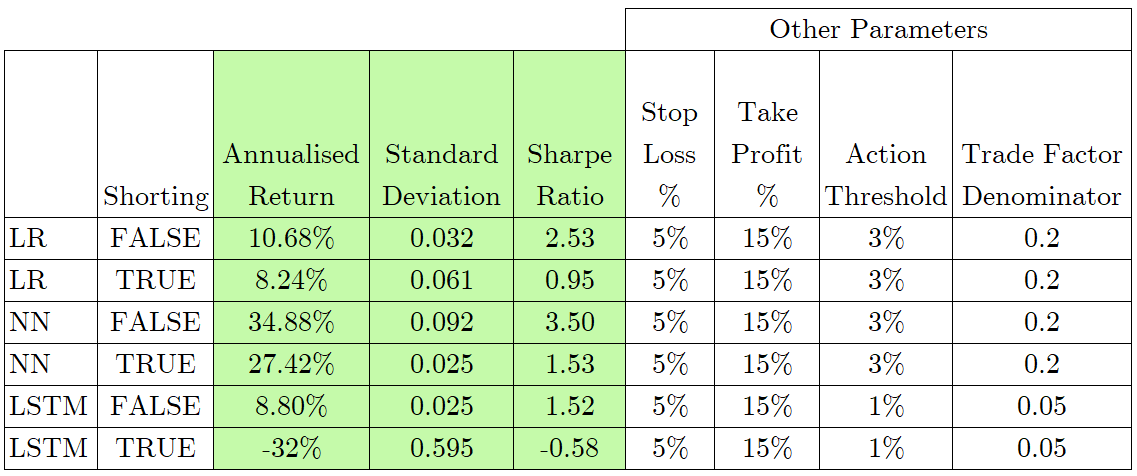
\includegraphics[width=16cm]{ML_results_comparison}}
  \caption{Comparision of Results for MLR/NN/LSTM}
  \label{fig:Comparison of Results}
\end{figure}
After the total portfolio value graph of each approach is generated, the Risk and Profitability measures are calculated with the formulas in Section 5.1.3.\\


From the results, it appears that trading without shorting is superior in terms of profitability and sharpe ratio. This is possibly because short selling creates the potential for unlimited losses (Bryant, 2023), because regardless of how high share prices rise, the investor will have to buy back the share to return to the market maker. \\

Surprisingly, the NN approach has the highest Sharpe Ratio of 3.5 followed by LR with 2.53 and LSTM with 1.52. This could be because of how the trade execution logic is devised, which requires the change predicted to be above the action threshold percentage. The changes predicted by the LSTM model are relatively small and hence much fewer trades are made resulting in less profits. Nevertheless, NN and MLR have resulted in a profitable trading strategy that minimises risk and maximises profits with a sharpe ratio greater than 2. 


\chapter{Alpha Tree Search Results}
\section{Alphas Generated}
The GA search of the Alpha Tree was run 5 times, with 20 iterations each and it generated the following high performing alphas:
\begin{figure}[H]
  \centerline{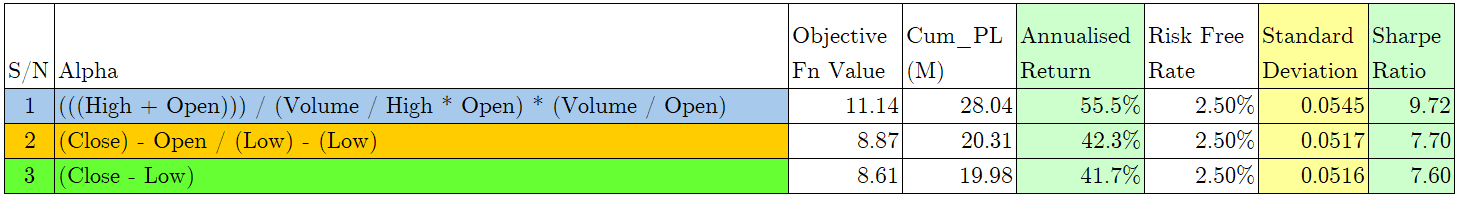
\includegraphics[width=20cm]{generated_alphas}}
  \caption{Top 3 Results from Alpha Tree Search}
  \label{fig:alphas_generated}
\end{figure}

\section{Portfolio Allocation Results with Best Performing Alphas}

\begin{figure}[H]
  \centerline{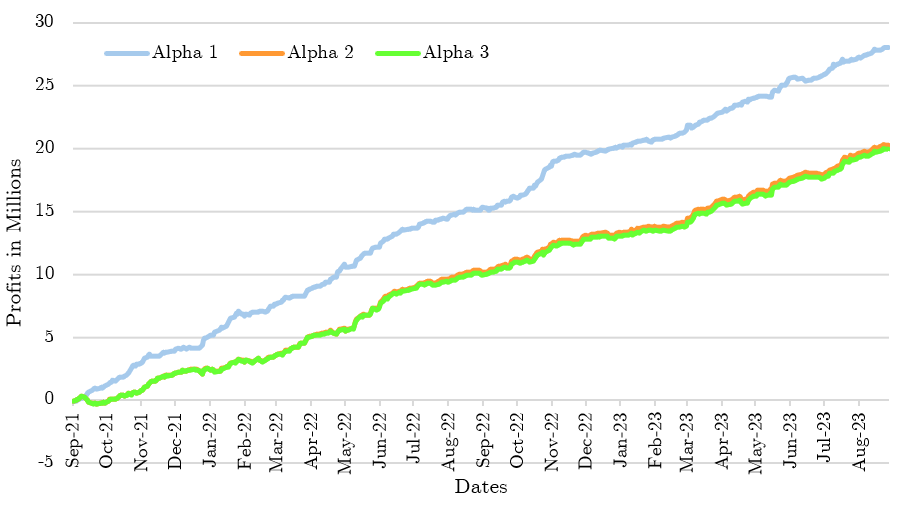
\includegraphics[width=15cm]{Alphas Profit Over Time}}
  \caption{Cumulative PnL for Top 3 Alphas}
  \label{fig:pnl_top_3}
\end{figure}
All 3 top performing Alphas resulting from the Genetic Algorithm have a high sharpe ratio of 11.14, 8.87 and 8.61. and annualised return of 55.5\%, 42.3\% and 41.7\% respectively (Figure \ref{fig:alphas_generated}) and a strong and consistently growing profit over the years (Figure \ref{fig:pnl_top_3}). \\

Using a starting investment capital of 20 Million dollars, all three Alphas managed to reap more than 100\% returns over a 3 year period demonstrating the strength of the GA technique of searching for outperforming Alphas. Moreover, the risk is maintained at a relatively low level at a 5\% standard deviation. This suggests that even in the worst case scenarios trading with these Alphas would still generate strong supernormal profits.


\chapter{Conclusion}
This section summarises the approaches by comparing them against the average REIT stock, industry benchmarks i.e. the REIT market indexes and traditional measures like ARIMA and GARCH. It will then compare the key characteristics of the models and summarise the key findings of the project. 
\section{Benchmarking Against Indexes, ARIMA, GARCH}
\begin{figure}[H]
  \centerline{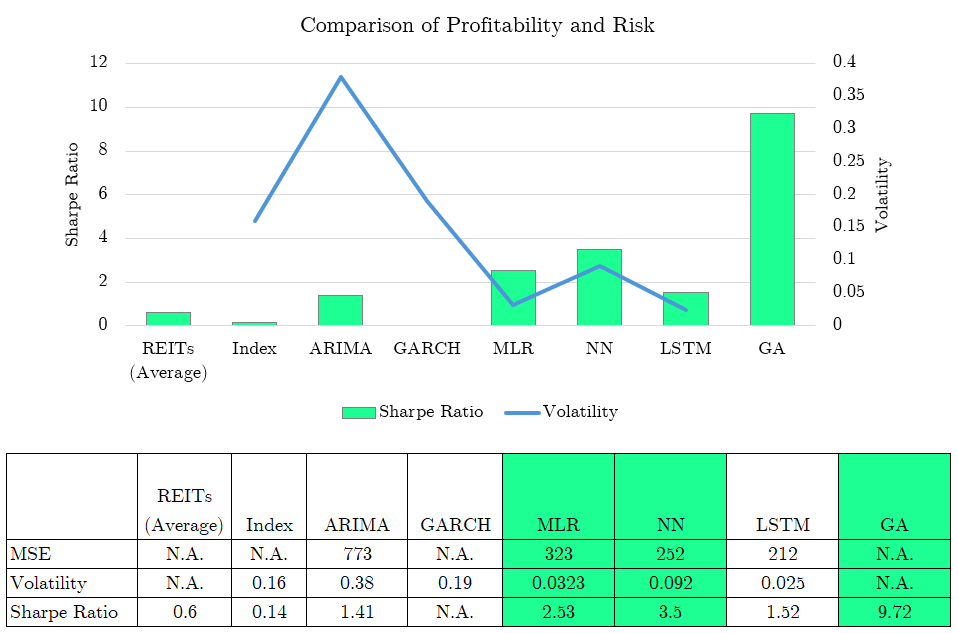
\includegraphics[width=18cm]{final comparison}}
  \caption{Benchmarking This Paper's Approaches}
  \label{fig:final_comparison}
\end{figure}

From Figure \ref{fig:final_comparison}, it appears that ML models significantly outperform traditional approaches to portfolio optimisation with more than double the sharpe ratio. The Genetic Algorithm especially outperforms with its high sharpe ratio of 9.72 compared to the market index of 0.14 or the average REIT stock of 0.6. In terms of risk and volatility, the ML models also have significantly lower volatity than the market index and ARIMA as represented by the blue line.







\section{Comparing Characteristics of Approaches}
\begin{figure}[H]
  \centerline{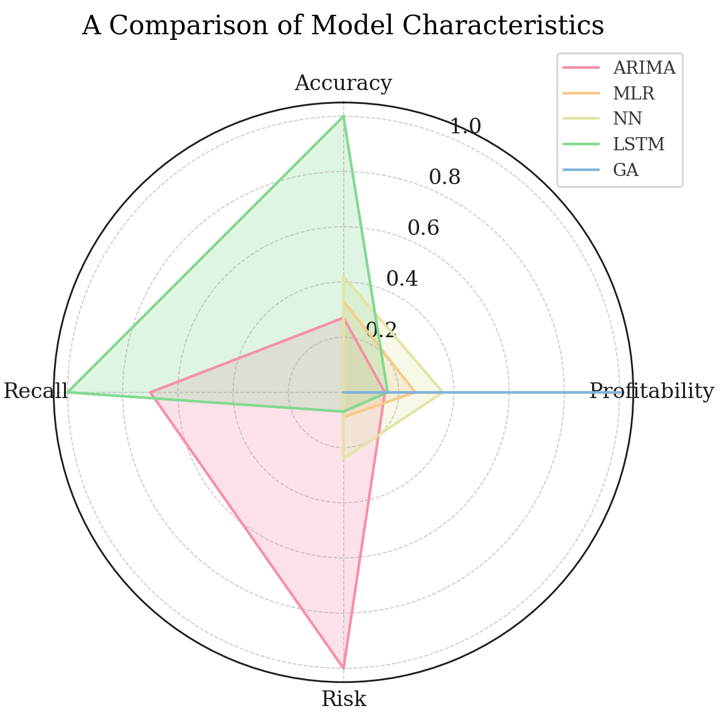
\includegraphics[width=15cm]{Final Comparsion of Models}}
  \caption{Comparing Approaches on Profitability, Risk, Accuracy and Recall}
  \label{fig:final_comparison_of_models}
\end{figure}

The spider web chart in Figure \ref{fig:final_comparison_of_models} compares the strengths and weaknesses of this paper's approaches and the traditional ARIMA. \\

GA significantly outperforms all other methods in terms of Profitability and the ML applications adopted in this paper have generally greater profit and lower risk than the index and ARIMA. Although LSTM only has average profitability it is one of the few approaches like ARIMA with an ability to recall and incorporate a window of past data. LSTM also has the highest predictive accuracy followed by NN. 

\section{Key Findings}
The key findings for this paper are as follows:
\begin{enumerate}
  \item {The novel application of Genetic Algorithms to search for outperforming Alphas is successful and performs well in optimising real estate portfolios. It results in profitability that well exceeds the market average while minimising risk.}
  \item {The extension of input data for ML models to include fundamental data results in acceptable predictions and portfolio returns that have a sharpe ratio of more than 2 for NN and LR approaches. }
  \item {As whole the ML approaches and GA approach adopted by this paper outperforms the traditional and market approaches.}
  \item {It is surprising that despite LSTM's highest accuracy in predicting the next day's closing price, the portfolio allocation based on LSTM's predictions perform the poorest. This emphasises that for the ML models, the trade execution logic that implements the actual portfolio allocation based on predictions has a large effect on the overall portfolio performance beyond price prediction.  }
\end{enumerate}

\section{Major Contribution and Creativity}
This paper demonstrated creativity by:
\begin{enumerate}
  \item {Combining the ideas of Genetic Algorithms and Alphas to REITs, and writing a new search algorithm that managed to find outperforming Alpha formulas to optimise the allocation of Real Estate Portfolios.}
  \item {Incorporating fundamental analysis into ML models beyond the usual technical analysis done by most papers in the field.}
\end{enumerate}

Moreover this Paper's main contribution are:
\begin{enumerate}
  \item {Real Estate Portfolio Optimisation Strategies using GA and ML approaches that maximise profits and minimise risk that significantly outperform the market with a sharpe ratio greater than 2.}
  \item {The Python code for the GA Search Algorithm}
  \item {The implementation and Python code of the trading agent and trade excecution logic that does portfolio allocation based on predicted prices from ML models. Most papers (as seen in the literature review) focus on price prediction, but this paper also contributes the mechanism for portfolio optimisation.}
  \item {ML on Fundamental Data with 20+ feateures for 150 Tickers for the past 20 years. A dataste that covers more than 20\% of all REITs in the world, making this study especially representative. Also providing the directions to purchase this data at an affordable price for future research.}
\end{enumerate}

\section{Future Work}

The Genetic Algorithm approach has great room for exploration. This paper's code only uses 4 basic operators, but many more operators such as ranking, correlation etc can be passed into the code to enhance the permutation of generated Alphas. In addition, more valid datafields can be added to the GA code to create a wider range of Alphas.\\

As observed in this paper, the trade execution logic has a large impact on the overall profitability of the portfolio allocation for ML price prediction approaches. Hence, more experiments can be done with regards to the various parameters input into the trade execution code, and possibly refine the logic to improve performance. It is also conceivable that trade execution can be done with a Reinforcement Learning agent.

\pagebreak

hi
\cite{sheth_predicting_2023}
\cite{obthong_survey_2020}
\cite{habbab_-depth_2024}
\cite{tostevin_total_2023}
\cite{nareit_global_2024}
\cite{oberlechner_importance_2001}
\cite{tulchinsky_finding_2019}
\cite{wang_alpha-gpt_2023}
\cite{ruse_charles_1975}
\cite{aguilar-rivera_genetic_2015}
\cite{tulchinsky_finding_2019}
\cite{kakushadze_101_2016}
\cite{alexandria_unlocking_2023}
\cite{ross_fundamentals_2021} 
\cite{ariyo_stock_2014}
\cite{habbab_machine_2022}
\cite{obthong_survey_2020} 
\cite{fiszeder_what_2020}
\cite{lama_modelling_2015}
\cite{yuan_garch_2017}
\cite{shakhla_stock_2020}
\cite{dey_comparative_2021} 
\cite{axelsson_univariate_2023}
\cite{cao_fundamental_2021}
\cite{huang_machine_2021}  
\citep{bryant_why_2023}



\bibliographystyle{plain}
\bibliography{references}

\end{document}


